% Typ des Dokuments
\documentclass[abstracton, a4paper, 12pt]{scrreprt}

% Encoding (utf8)
\usepackage[utf8]{inputenc}
\usepackage[T1]{fontenc}

% Silbentrennung (Neu-Deutsch)
\usepackage[ngerman]{babel}

% Literaturverzeichnis (Deutsch)
\usepackage{bibgerm}
% Spezialseiten (Literarturverzeichnis, Abbildungsverzeichnis, usw.) in Inhaltsverzeichnis anzeigen
\usepackage[nottoc]{tocbibind}

% Farben
\usepackage{color}
\usepackage[table]{xcolor}
\definecolor{darkgreen}{rgb}{0,0.6,0}
\definecolor{darkgrey}{rgb}{0.5,0.5,0.5}
\definecolor{grey}{rgb}{0.8,0.8,0.8}
\definecolor{lightgrey}{rgb}{0.95,0.95,0.95}
\definecolor{mauve}{rgb}{0.58,0,0.82}

% Schriften
\usepackage{pifont}
\newcommand{\tick}{\ding{51}\hspace{0.2cm}}
\newcommand{\cross}{\ding{55}\hspace{0.2cm}}

% Grafiken
\usepackage[pdftex]{graphicx}
\usepackage{epsfig}
% Umfliessen von Text um Tabellen und Bilder
\usepackage{wrapfig}

% PDFs
\usepackage{pdfpages}

% Grafiken korrekt positionieren
\usepackage{float}
\restylefloat{figure}
\usepackage[section]{placeins}
\usepackage{subfigure}
% Zahlen verwenden für Subfigure counter
\renewcommand{\thesubfigure}{(\arabic{subfigure})}

% Hyperlinks und URLs
\usepackage[hyphens]{url}
\usepackage{hyperref}
\hypersetup{
   colorlinks,%
   citecolor=[rgb]{0,0.35,0.9},%
   filecolor=[rgb]{0,0.35,0.9},%
   linkcolor=[rgb]{0,0.35,0.9},%
   urlcolor=[rgb]{0,0.35,0.9}
}
\urlstyle{same}

% Absatz
\setlength{\parindent}{0pt} % Absatzeinzug
\setlength{\parskip}{10pt} % Absatzabstand

% Glossar
\usepackage[toc]{glossaries}
\makeglossary

% Kontrolle über Listen-Eigenschaften
\usepackage{enumitem}

% Abstaende bei Ueberschriften
\usepackage{titlesec}
% \titlespacing*{command}{left}{before-sep}{after-sep}[right-sep]
\titlespacing{\section}{0em}{12pt}{3pt}
\titlespacing{\subsection}{0em}{10pt}{2pt}
\titlespacing{\subsubsection}{0em}{8pt}{0em}

% TODO Kommentare
\usepackage{todonotes}

%%%%%%%%%%%%%%%%%%%%%%%%%%%%%%%%%%%%%%%%%%%%%%%%%%%
% Kopf- und Fusszeile
%%%%%%%%%%%%%%%%%%%%%%%%%%%%%%%%%%%%%%%%%%%%%%%%%%%
% Seitenränder
\usepackage[inner=2.2cm,outer=2.2cm,top=1.7cm,bottom=1.7cm,includeheadfoot]{geometry}

% Kopf- und Fusszeile mit Linien
\usepackage[automark,headsepline,footsepline]{scrpage2}

\pagestyle{scrheadings}
% Kopf- und Fusszeile auch bei Kapitel- und Partsanfangsseiten
\renewcommand*{\chapterpagestyle}{scrheadings}
\renewcommand*{\partpagestyle}{scrheadings} 

% Kopf- und Fusszeile leeren
\clearscrheadfoot

% Inhalt der Kopfzeile
\ihead{\footnotesize{\leftmark}}

% Inhalt der Fusszeile
\ifoot{\footnotesize{Kort Reloaded – A Gamified App for Collecting OpenStreetMap Data}}
\ofoot{\footnotesize{\thepage}}

% MakeUppercase überschreiben, um Grosschreibung in Kopfzeile für Spezialseiten zu deaktivieren (Achtung böser Hack!)
\renewcommand*\MakeUppercase[1]{#1}

%%%%%%%%%%%%%%%%%%%%%%%%%%%%%%%%%%%%%%%%%%%%%%%%%%%
% Tabellen
%%%%%%%%%%%%%%%%%%%%%%%%%%%%%%%%%%%%%%%%%%%%%%%%%%%
% Für Tabellen, welche über mehrere Seiten gehen
\usepackage{longtable}

% Mehrere Spalten zusammenfassen
\usepackage{hhline}

% Mehrere Zeilen zusammenfassen
% \usepackage{multirow}
\usepackage{array}

% Tabularx
\usepackage{tabularx, booktabs}

% Padding links und rechts von Zelle
\setlength{\tabcolsep}{5px}
% Padding oben und unten (mittels arraystretch)
\renewcommand{\arraystretch}{1.3}

% Variabeln für Tabellenbreiten definieren
% 2-spaltige Tabelle
\newlength{\twocelltabwidth}
\setlength{\twocelltabwidth}{\textwidth}
\addtolength{\twocelltabwidth}{-4\tabcolsep - 3px} % subtrahiere 4x Padding (\tabcolsep) und 3 Rahmen

% 3-spaltige Tabelle
\newlength{\threecelltabwidth}
\setlength{\threecelltabwidth}{\textwidth}
\addtolength{\threecelltabwidth}{-6\tabcolsep - 4px} % subtrahiere Padding (\tabcolsep) und Rahmen

% 4-spaltige Tabelle
\newlength{\fourcelltabwidth}
\setlength{\fourcelltabwidth}{\textwidth}
\addtolength{\fourcelltabwidth}{-8\tabcolsep - 5px} % subtrahiere Padding (\tabcolsep) und Rahmen

%%%%%%%%%%%%%%%%%%%%%%%%%%%%%%%%%%%%%%%%%%%%%%%%%%%
% Syntaxhighlighter
%%%%%%%%%%%%%%%%%%%%%%%%%%%%%%%%%%%%%%%%%%%%%%%%%%%
% Syntaxhighlighter (benoetigt color und xcolor package)
\usepackage{listings}
\renewcommand{\lstlistingname}{Code-Ausschnitt}

\lstset{ %
  language=HTML,                % the language of the code
  basicstyle=\footnotesize,           % the size of the fonts that are used for the code
  numbers=left,                   % where to put the line-numbers
  numberstyle=\tiny\color{darkgrey},  % the style that is used for the line-numbers
  stepnumber=1,                   % the step between two line-numbers. If it's 1, each line will be numbered
  numbersep=5pt,                  % how far the line-numbers are from the code
  backgroundcolor=\color{white},  % choose the background color. You must add \usepackage{color}
  showspaces=false,               % show spaces adding particular underscores
  showstringspaces=false,         % underline spaces within strings
  showtabs=false,                 % show tabs within strings adding particular underscores
  frame=single,                   % adds a frame around the code
  rulecolor=\color{darkgrey},        % if not set, the frame-color may be changed on line-breaks within not-black text (e.g. commens (green here))
  tabsize=2,                      % sets default tabsize to 2 spaces
  captionpos=b,                   % sets the caption-position to bottom
  breaklines=true,                % sets automatic line breaking
  breakatwhitespace=false,        % sets if automatic breaks should only happen at whitespace
  title=\lstname,                   % show the filename of files included with \lstinputlisting;
                                  % also try caption instead of title
  keywordstyle=\color{blue},          % keyword style
  commentstyle=\color{darkgreen},       % comment style
  stringstyle=\color{mauve},         % string literal style
  escapeinside={\%*}{*)},            % if you want to add a comment within your code
  morekeywords={*,...}               % if you want to add more keywords to the set
}

% Javascript Syntaxhighliting
\lstdefinelanguage{JavaScript} {
	morekeywords={
		break,const,continue,delete,do,while,export,for,in,function,
		if,else,import,in,instanceOf,label,let,new,return,switch,this,
		throw,try,catch,typeof,var,void,with,yield
	},
	sensitive=false,
	morecomment=[l]{//},
	morecomment=[s]{/*}{*/},
	morestring=[b]",
	morestring=[d]'
}
\lstset{
	frame=tb,
	framesep=5pt,
	basicstyle=\footnotesize\ttfamily,
	showstringspaces=false,
	keywordstyle=\ttfamily\bfseries\color{blue},
	identifierstyle=\ttfamily,
	stringstyle=\ttfamily\color{mauve},
	commentstyle=\color{darkgreen},
	rulecolor=\color{darkgrey},
	xleftmargin=5pt,
	xrightmargin=5pt,
	aboveskip=\bigskipamount,
	belowskip=\bigskipamount
}

\lstdefinestyle{examples}
{numbers=none, frame=none}

% Inline Code-Formatierung
\newcommand{\inlinecode}{\texttt}

% Applikationsname Kort
\newcommand\kort{\textsc{Kort}}

% Marken- oder Produktnamen
\newcommand\brand{\emph}

% Silbentrennung
\hyphenation{Web-app-li-ka-tion}
\hyphenation{Ja-va-Scr-ipt}

% Tree Package
% CD-Inhalt
\usepackage{forest}
\definecolor{root}{RGB}{45,62,135}
\definecolor{edge}{RGB}{52,72,154}
\definecolor{folder1}{RGB}{46,68,150}
\definecolor{folder2}{RGB}{53,74,165}
\definecolor{folder3}{RGB}{59,81,180}
\definecolor{folder4}{RGB}{64,88,195}
\definecolor{file}{RGB}{96,115,205}
% Glossar
\newglossaryentry{NativeApp} {
	name = Native App,
	description = {Native Apps im engeren Sinn zeichnen sich dadurch aus, dass sie speziell an die Zielplattform angepasst und sehr leicht über ein herstellerspezifisches Online-Portal bezogen und installiert werden können\cite{mobileapp}}
}

\newglossaryentry{API} {
	name = API,
	description = {Application Programming Interface, Schnittstelle für die Programmierung\cite{ba-kort-2012}}
}

\newglossaryentry{OAuth} {
	name = OAuth,
	description = {OAuth ist ein offenes Protokoll, das eine standardisierte, sichere API-Autorisierung erlaubt\cite{oauth}}
}

\newglossaryentry{CRUD} {
	name = CRUD,
	description = {Das Akronym CRUD beschreibt die 4 Standardoperationen einer Datenbank: \textbf{C}reate, \textbf{R}ead, \textbf{U}pdate, \textbf{D}elete\cite{crud}}
}

\newglossaryentry{WebApp} {
	name = Web-App,
	description = {Der Begriff Web-App (von der englischen Kurzform für web application) bezeichnet im allgemeinen Sprachgebrauch Apps für mobile Endgeräte wie Smartphones und Tablet-Computer. 
	Diese Apps laufen auf dem im Betriebssystem integrierten Browser, werden aus dem Internet geladen und können so ohne Installation auf dem mobilen Endgerät genutzt werden\cite{webapp}}
}

\newglossaryentry{REST} {
	name = REST,
	description = {Representational State Transfer\cite{rest} ist ein Programmierparadigma, welches besagt, dass sich der Zustand einer Webapplikation als Ressource in Form einer URL beschreiben lässt. Auf solche Ressourcen können folgende Befehle angewendet werden: \inlinecode{GET}, \inlinecode{POST}, \inlinecode{PUT}, \inlinecode{PATCH}, \inlinecode{DELETE}, \inlinecode{HEAD} und \inlinecode{OPTIONS}.
	HTTP ist ein Protokoll welches REST implementiert\cite{ba-kort-2012}}
}

\newglossaryentry{Git} {
	name = Git,
	description = {Git ist ein verteiltes Versionsverwaltungssystem für Dateien. Ursprünglich wurde es für die Entwicklung des Linux Kernels kreiert\cite{ba-kort-2012}}
}

\newglossaryentry{CI} {
	name = Continuous Integration,
	description = {Der Begriff \emph{Continuous Integration}\cite{cont-integration} beschreibt die Idee, dass Änderungen an einer Software schnell eingebracht werden sollen. Dazu zählt, dass diese in einem Tool zur Versionsverwaltung eingetragen und durch automatisierte Tests geprüft werden\cite{ba-kort-2012}}
}

\newglossaryentry{POI} {
	name = POI,
	description = {Abkürzung für Point of Interest. Dies ist ein allgemeiner Begriff für einen Ort mit irgendeiner Bedeutung, sei es eine Schule, Kirche, Bushaltestelle oder sonst etwas von besonderem Interesse\cite{ba-kort-2012}}
}

\newglossaryentry{Mapper} {
	name = Mapper,
	description = {Personen welche auf OpenStreetMap die Karten ergänzen und pflegen, nennen sich selbst \emph{Mapper}\cite{ba-kort-2012}}
}

\newglossaryentry{App Store} {
	name = App Store,
	description = {Ein App Store ist eine Verkaufsplattform eines Betriebssystemherstellers für Smartphones, beispielsweise Google Play für Android, Apple App Store für iOS\cite{ba-kort-2012}}
}

\newglossaryentry{Node} {
	name = Node,
	description = {Ein Node ist das grundlegendste Objekt in OpenStreetMap, es wird durch seine Attribute (genannt \glspl{Tag}) genauer bestimmt. Nodes können Teil eines \gls{Way} sein\cite{ba-kort-2012}}
}

\newglossaryentry{Way} {
	name = Way,
	description = {Ein Weg oder eine Strasse wird in OpenStreetMap als \emph{Way} bezeichnet. Es handelt sich dabei um eine Serie von miteinander verbundenen Nodes\cite{ba-kort-2012}}
}

\newglossaryentry{Relation} {
	name = Relation,
	description = {Eine Relation stellt eine Verbindung zwischen verschiedenen OSM-Objekten dar. Relationen werden meist dazu gebraucht, um übergeordnete Beziehungen darzustellen. Beispielsweise können alle Bushaltestellen einer Buslinie über eine Relation miteinander verknüpft sein\cite{ba-kort-2012}}
}

\newglossaryentry{Tag} {
	name = Tag,
	description = {Ein Tag bezeichnet ein Attribut eines \glslink{Node}{Nodes}. Es besteht aus einem Namen und einem Wert. Ein \gls{Node} kann beliebig viele Tags beinhalten\cite{ba-kort-2012}}
}

\newglossaryentry{OpenStreetMap} {
	name = OpenStreetMap,
	description = {OpenStreetMap ist ein freies Projekt, das für jeden frei nutzbare Geodaten sammelt (Open Data). Mit Hilfe dieser Daten können Weltkarten errechnet oder Spezialkarten abgeleitet werden sowie Navigation betrieben werden\cite{ba-kort-2012}}
}

\newglossaryentry{Gamification} {
	name = Gamification,
	description = {Unter Gamification versteht man das Hinzufügen von Spielelementen in einen nicht spieltypischen Kontext.\cite{for-the-win}}
}

\newglossaryentry{MVC} {
	name = MVC,
	description = {Der englischsprachige Begriff \emph{model view controller} (MVC) ist ein Muster zur Strukturierung von Software-Entwicklung in die drei Einheiten Datenmodell (model), Präsentation (view) und Programmsteuerung (controller)\cite{patterns}}
}

\newglossaryentry{Crowdsourcing} {
	name = Crowdsourcing,
	description = {Unter Crowdsourcing versteht man die Auslagerung von traditionell internen Teilaufgaben an eine Menge von freiwilligen Usern im Internet\cite{crowdsourcing}}
}

\newglossaryentry{Routing} {
	name = Routing,
	description = {Routing beschreibt den Vorgang einen optimalen Weg zwischen zwei oder mehr Punkten zu finden. Eine so gefundene Strecke wird oft als \emph{Route} bezeichnet\cite{ba-kort-2012}}
}

\newglossaryentry{Pair Programming}{
	name = Pair Programming,
	description = {Bei Pair Programming handelt es sich um eine Arbeitsweise, bei der zwei Programmierer an einem Rechner arbeiten. Dabei ist ein Programmierer damit beschäftigt, den Code zu schreiben, während der andere über die Problemstellungen nachdenkt, den geschriebenen Code kontrolliert und Probleme, die ihm dabei auffallen, sofort anspricht\cite{pairprogramming}}
}

\newglossaryentry{Minimum Viable Product}{
	name = Minimum Viable Product,
	description = {Das Minimum Viable Product ist ein Produkt, welches gerade die Kernfunktionalität aufweist, die nötig ist um es zu veröffentlichen\cite{mvp}}
}

\newglossaryentry{Framework}{
	name = Framework,
	description = {Ein Framework ist noch kein fertiges Programm. 
	Es ist ein Rahmen (ein Gerüst) welches der Programmierer verwenden kann um sein eigenes, persönliches Programm zu erstellen\cite{framework}}
}

\newglossaryentry{GUI}{
	name = GUI,
	description = {GUI ist eine Abkürzung für graphical user interface und bedeutet grafische Benutzer-oberfläche\cite{gui}}
}

\newglossaryentry{Library}{
	name = Library,
	description = {Eine Library (Programmbibliothek) bezeichnet in der Programmierung eine Sammlung von Unterprogrammen, die Lösungswege anbieten. 
	Bibliotheken laufen im Unterschied zu Programmen nicht eigenständig, sondern sie enthalten Hilfsmodule, die angefordert werden können\cite{library}},
	plural= Libraries
}

\newglossaryentry{DOM}{
	name = DOM,
	description = {DOM bedeutet Document Object Model und ist eine Spezifikation für den Zugriff auf HTML-Dokumente. 
	Anhand des DOMs kann ein Computerprogramm den Inhalt der HTML-Elemente dynamisch verändern. 
	Für einen Webentwickler wäre das der HTML-Code.\cite{dom}}
}

\newglossaryentry{Virtual DOM}{
	name = Virtual DOM,
	description = {Das virtual DOM ist eine Abstraktion des DOM. 
	Es ist eine lokale Kopie des DOM\cite{virtual-dom}}
}

\newglossaryentry{JSX}{
	name = JSX,
	description = {JSX ist eine \brand{JavaScript}-Syntax-Erweiterung die ähnlich wie XML aussieht\cite{jsx}}
}

\newglossaryentry{Backend}{
	name = Backend,
	description = {Als Backend wird das auf dem Server laufenden Programm bezeichnet}
}

\newglossaryentry{Frontend}{
	name = Frontend,
	description = {Als Frontend wird das beim Client laufende Programm bezeichnet}
}

\newglossaryentry{DTO}{
	name = DTO,
	description = {Ein Datentransferobjekt ist ein Objekt, das nur zur Übertragung von Daten oder Informationen dient und keine logischen Komponenten enthält}
}

\newglossaryentry{Singleton}{
	name = Singleton,
	description = {Das Singleton beschreibt ein Entwurfsmuster, wonach sichergestellt wird, dass von einer Klasse immer höchstens ein Objekt existiert, welches üblicherweise global verfügbar ist\cite{singleton}}
}

\newglossaryentry{IDE}{
	name = IDE,
	description = {IDE bedeutet Integrierte Entwicklungsumgebung -- auf Englisch integrated development environment\cite{ide}}
}

\newglossaryentry{Unit Test}{
	name = Unit Test,
	description = {Unit Tests werden geschrieben um kleine Teile des Codes -- üblicherweise Module -- zu testen.
	Da wirklich nur das Verhalten des entsprechenden Moduls getestet werden soll, müssen Abhängigkeiten dieses Moduls durch \glslink{Mock}{Mocks} ersetzt werden}
}

\newglossaryentry{Integration Test}{
	name = Integration Test,
	description = {In Integration Tests wird die Zusammenarbeit von Systemteilen getestet}
}

\newglossaryentry{Funktionaler Test}{
	name = Funktionaler Test,
	description = {Funktionale Tests überprüfen das Gesamtverhalten des Systems.
	Mit einem automatisierten UI Testing Tool werden verschiedene Szenarien durchlaufen, welche aus den Use Cases abgeleitet werden können.
	Funktionale Tests werden im Vergleich zu \glslink{Unit Test}{Unit Tests} und \glslink{Integration Test}{Integration Tests} eher spärlich eingesetzt}
}
	
\newglossaryentry{Mock}{
	name = Mock,
	description = {Mock-Objekte werden in diversen Tests verwendet um das Verhalten eines anderen Objekts für spezifische Fälle zu simulieren ohne es tatsächlich zu implementieren}
} 

\newglossaryentry{Packager}{
	name = Packager,
	description = {Der Packager kompiliert und bundelt den JavaScript Code für das Smartphone während der Entwicklungsphase und dem Testen auf dem Gerät}
} 
\begin{document}

% ToDo Liste


% -----------------------------------------
% HEAD
% -----------------------------------------
% Titelseite
\title{Kort Reloaded – A Gamified App for Collecting OpenStreetMap Data}
\author{Marino Melchiori
		\and
		Dominic Mülhaupt}
%\date{10. März 2016}

\begin{titlepage}

% Logos
\begin{figure}[H]
\subfigure{
\includegraphics[width=200px]{images/titelseite/logo-hsr}}
\hfill
\raisebox{24px}{\subfigure{
\includegraphics[width=125px]{images/titelseite/logo-liip}}}
\end{figure}

\vspace{2cm}

\begin{center}
{ \Large
	% Titel
	\textbf{Kort Reloaded -- A Gamified App for Collecting OpenStreetMap Data}
	\vspace{1cm}

	% Arbeitstyp / Schule
	\textbf{Bachelorarbeit}
	\vspace{1cm}

	Abteilung Informatik \\[0.2cm]
	HSR Hochschule für Technik Rapperswil
	\vspace{1cm}

	% Semester
	Frühjahrssemester 2016
}
\end{center}
\vspace{1cm}


\begin{table}[H] 
\centering 
\begin{tabular}{p{0.19\twocelltabwidth}p{0.4\twocelltabwidth}}
Autoren: & \textbf{Marino Melchiori} \newline
\textbf{Dominic Mülhaupt} \\ 
Betreuer: & \textbf{Prof. Stefan Keller} \\ 
Projektpartner: & \textbf{Jürg Hunziker} \newline
\textbf{Stefan Oderbolz} \newline
Liip AG\\ 
Experte: & \textbf{Claude Eisenhut} \\ 
Gegenleser: & \textbf{Prof. Beat Stettler} \\ 
\end{tabular}
\end{table}

\end{titlepage}

% Seitennummerierung mit roemischen Zeichen
\pagenumbering{roman}

% Glossar (muss vor Body inkludiert werden, damit Referenzen funktionieren)
% Glossar
\newglossaryentry{NativeApp} {
	name = Native App,
	description = {Native Apps im engeren Sinn zeichnen sich dadurch aus, dass sie speziell an die Zielplattform angepasst und sehr leicht über ein herstellerspezifisches Online-Portal bezogen und installiert werden können\cite{mobileapp}}
}

\newglossaryentry{API} {
	name = API,
	description = {Application Programming Interface, Schnittstelle für die Programmierung\cite{ba-kort-2012}}
}

\newglossaryentry{OAuth} {
	name = OAuth,
	description = {OAuth ist ein offenes Protokoll, das eine standardisierte, sichere API-Autorisierung erlaubt\cite{oauth}}
}

\newglossaryentry{CRUD} {
	name = CRUD,
	description = {Das Akronym CRUD beschreibt die 4 Standardoperationen einer Datenbank: \textbf{C}reate, \textbf{R}ead, \textbf{U}pdate, \textbf{D}elete\cite{crud}}
}

\newglossaryentry{WebApp} {
	name = Web-App,
	description = {Der Begriff Web-App (von der englischen Kurzform für web application) bezeichnet im allgemeinen Sprachgebrauch Apps für mobile Endgeräte wie Smartphones und Tablet-Computer. 
	Diese Apps laufen auf dem im Betriebssystem integrierten Browser, werden aus dem Internet geladen und können so ohne Installation auf dem mobilen Endgerät genutzt werden\cite{webapp}}
}

\newglossaryentry{REST} {
	name = REST,
	description = {Representational State Transfer\cite{rest} ist ein Programmierparadigma, welches besagt, dass sich der Zustand einer Webapplikation als Ressource in Form einer URL beschreiben lässt. Auf solche Ressourcen können folgende Befehle angewendet werden: \inlinecode{GET}, \inlinecode{POST}, \inlinecode{PUT}, \inlinecode{PATCH}, \inlinecode{DELETE}, \inlinecode{HEAD} und \inlinecode{OPTIONS}.
	HTTP ist ein Protokoll welches REST implementiert\cite{ba-kort-2012}}
}

\newglossaryentry{Git} {
	name = Git,
	description = {Git ist ein verteiltes Versionsverwaltungssystem für Dateien. Ursprünglich wurde es für die Entwicklung des Linux Kernels kreiert\cite{ba-kort-2012}}
}

\newglossaryentry{CI} {
	name = Continuous Integration,
	description = {Der Begriff \emph{Continuous Integration}\cite{cont-integration} beschreibt die Idee, dass Änderungen an einer Software schnell eingebracht werden sollen. Dazu zählt, dass diese in einem Tool zur Versionsverwaltung eingetragen und durch automatisierte Tests geprüft werden\cite{ba-kort-2012}}
}

\newglossaryentry{POI} {
	name = POI,
	description = {Abkürzung für Point of Interest. Dies ist ein allgemeiner Begriff für einen Ort mit irgendeiner Bedeutung, sei es eine Schule, Kirche, Bushaltestelle oder sonst etwas von besonderem Interesse\cite{ba-kort-2012}}
}

\newglossaryentry{Mapper} {
	name = Mapper,
	description = {Personen welche auf OpenStreetMap die Karten ergänzen und pflegen, nennen sich selbst \emph{Mapper}\cite{ba-kort-2012}}
}

\newglossaryentry{App Store} {
	name = App Store,
	description = {Ein App Store ist eine Verkaufsplattform eines Betriebssystemherstellers für Smartphones, beispielsweise Google Play für Android, Apple App Store für iOS\cite{ba-kort-2012}}
}

\newglossaryentry{Node} {
	name = Node,
	description = {Ein Node ist das grundlegendste Objekt in OpenStreetMap, es wird durch seine Attribute (genannt \glspl{Tag}) genauer bestimmt. Nodes können Teil eines \gls{Way} sein\cite{ba-kort-2012}}
}

\newglossaryentry{Way} {
	name = Way,
	description = {Ein Weg oder eine Strasse wird in OpenStreetMap als \emph{Way} bezeichnet. Es handelt sich dabei um eine Serie von miteinander verbundenen Nodes\cite{ba-kort-2012}}
}

\newglossaryentry{Relation} {
	name = Relation,
	description = {Eine Relation stellt eine Verbindung zwischen verschiedenen OSM-Objekten dar. Relationen werden meist dazu gebraucht, um übergeordnete Beziehungen darzustellen. Beispielsweise können alle Bushaltestellen einer Buslinie über eine Relation miteinander verknüpft sein\cite{ba-kort-2012}}
}

\newglossaryentry{Tag} {
	name = Tag,
	description = {Ein Tag bezeichnet ein Attribut eines \glslink{Node}{Nodes}. Es besteht aus einem Namen und einem Wert. Ein \gls{Node} kann beliebig viele Tags beinhalten\cite{ba-kort-2012}}
}

\newglossaryentry{OpenStreetMap} {
	name = OpenStreetMap,
	description = {OpenStreetMap ist ein freies Projekt, das für jeden frei nutzbare Geodaten sammelt (Open Data). Mit Hilfe dieser Daten können Weltkarten errechnet oder Spezialkarten abgeleitet werden sowie Navigation betrieben werden\cite{ba-kort-2012}}
}

\newglossaryentry{Gamification} {
	name = Gamification,
	description = {Unter Gamification versteht man das Hinzufügen von Spielelementen in einen nicht spieltypischen Kontext.\cite{for-the-win}}
}

\newglossaryentry{MVC} {
	name = MVC,
	description = {Der englischsprachige Begriff \emph{model view controller} (MVC) ist ein Muster zur Strukturierung von Software-Entwicklung in die drei Einheiten Datenmodell (model), Präsentation (view) und Programmsteuerung (controller)\cite{patterns}}
}

\newglossaryentry{Crowdsourcing} {
	name = Crowdsourcing,
	description = {Unter Crowdsourcing versteht man die Auslagerung von traditionell internen Teilaufgaben an eine Menge von freiwilligen Usern im Internet\cite{crowdsourcing}}
}

\newglossaryentry{Routing} {
	name = Routing,
	description = {Routing beschreibt den Vorgang einen optimalen Weg zwischen zwei oder mehr Punkten zu finden. Eine so gefundene Strecke wird oft als \emph{Route} bezeichnet\cite{ba-kort-2012}}
}

\newglossaryentry{Pair Programming}{
	name = Pair Programming,
	description = {Bei Pair Programming handelt es sich um eine Arbeitsweise, bei der zwei Programmierer an einem Rechner arbeiten. Dabei ist ein Programmierer damit beschäftigt, den Code zu schreiben, während der andere über die Problemstellungen nachdenkt, den geschriebenen Code kontrolliert und Probleme, die ihm dabei auffallen, sofort anspricht\cite{pairprogramming}}
}

\newglossaryentry{Minimum Viable Product}{
	name = Minimum Viable Product,
	description = {Das Minimum Viable Product ist ein Produkt, welches gerade die Kernfunktionalität aufweist, die nötig ist um es zu veröffentlichen\cite{mvp}}
}

\newglossaryentry{Framework}{
	name = Framework,
	description = {Ein Framework ist noch kein fertiges Programm. 
	Es ist ein Rahmen (ein Gerüst) welches der Programmierer verwenden kann um sein eigenes, persönliches Programm zu erstellen\cite{framework}}
}

\newglossaryentry{GUI}{
	name = GUI,
	description = {GUI ist eine Abkürzung für graphical user interface und bedeutet grafische Benutzer-oberfläche\cite{gui}}
}

\newglossaryentry{Library}{
	name = Library,
	description = {Eine Library (Programmbibliothek) bezeichnet in der Programmierung eine Sammlung von Unterprogrammen, die Lösungswege anbieten. 
	Bibliotheken laufen im Unterschied zu Programmen nicht eigenständig, sondern sie enthalten Hilfsmodule, die angefordert werden können\cite{library}},
	plural= Libraries
}

\newglossaryentry{DOM}{
	name = DOM,
	description = {DOM bedeutet Document Object Model und ist eine Spezifikation für den Zugriff auf HTML-Dokumente. 
	Anhand des DOMs kann ein Computerprogramm den Inhalt der HTML-Elemente dynamisch verändern. 
	Für einen Webentwickler wäre das der HTML-Code.\cite{dom}}
}

\newglossaryentry{Virtual DOM}{
	name = Virtual DOM,
	description = {Das virtual DOM ist eine Abstraktion des DOM. 
	Es ist eine lokale Kopie des DOM\cite{virtual-dom}}
}

\newglossaryentry{JSX}{
	name = JSX,
	description = {JSX ist eine \brand{JavaScript}-Syntax-Erweiterung die ähnlich wie XML aussieht\cite{jsx}}
}

\newglossaryentry{Backend}{
	name = Backend,
	description = {Als Backend wird das auf dem Server laufenden Programm bezeichnet}
}

\newglossaryentry{Frontend}{
	name = Frontend,
	description = {Als Frontend wird das beim Client laufende Programm bezeichnet}
}

\newglossaryentry{DTO}{
	name = DTO,
	description = {Ein Datentransferobjekt ist ein Objekt, das nur zur Übertragung von Daten oder Informationen dient und keine logischen Komponenten enthält}
}

\newglossaryentry{Singleton}{
	name = Singleton,
	description = {Das Singleton beschreibt ein Entwurfsmuster, wonach sichergestellt wird, dass von einer Klasse immer höchstens ein Objekt existiert, welches üblicherweise global verfügbar ist\cite{singleton}}
}

\newglossaryentry{IDE}{
	name = IDE,
	description = {IDE bedeutet Integrierte Entwicklungsumgebung -- auf Englisch integrated development environment\cite{ide}}
}

\newglossaryentry{Unit Test}{
	name = Unit Test,
	description = {Unit Tests werden geschrieben um kleine Teile des Codes -- üblicherweise Module -- zu testen.
	Da wirklich nur das Verhalten des entsprechenden Moduls getestet werden soll, müssen Abhängigkeiten dieses Moduls durch \glslink{Mock}{Mocks} ersetzt werden}
}

\newglossaryentry{Integration Test}{
	name = Integration Test,
	description = {In Integration Tests wird die Zusammenarbeit von Systemteilen getestet}
}

\newglossaryentry{Funktionaler Test}{
	name = Funktionaler Test,
	description = {Funktionale Tests überprüfen das Gesamtverhalten des Systems.
	Mit einem automatisierten UI Testing Tool werden verschiedene Szenarien durchlaufen, welche aus den Use Cases abgeleitet werden können.
	Funktionale Tests werden im Vergleich zu \glslink{Unit Test}{Unit Tests} und \glslink{Integration Test}{Integration Tests} eher spärlich eingesetzt}
}
	
\newglossaryentry{Mock}{
	name = Mock,
	description = {Mock-Objekte werden in diversen Tests verwendet um das Verhalten eines anderen Objekts für spezifische Fälle zu simulieren ohne es tatsächlich zu implementieren}
} 

\newglossaryentry{Packager}{
	name = Packager,
	description = {Der Packager kompiliert und bundelt den JavaScript Code für das Smartphone während der Entwicklungsphase und dem Testen auf dem Gerät}
} 

% Impressum
\chapter*{Impressum}
% Titel auch in Kopfzeile anzeigen
\markboth{Impressum}{Impressum}

% Impressum
\begin{table}[H] 
\centering 
\begin{tabular}{|p{0.35\twocelltabwidth}|p{0.65\twocelltabwidth}|}
\hline 
\textbf{Autoren:} & Marino Melchiori (\url{mmelchio@hsr.ch}) \newline
Dominic Mülhaupt (\url{dmuelhau@hsr.ch}) \\ 
\hline 
\textbf{Dokument erstellt:} & 10.03.2016 \\ 
\hline 
\textbf{Letzte Aktualisierung:} & 28.06.2016 \\ 
\hline 
\end{tabular}
\end{table}

Dieses Dokument wurde mit \LaTeX{} erstellt.

% Erklaerung
%\chapter*{Eigenständigkeitserklärung}
% Titel auch in Kopfzeile anzeigen
\markboth{Eigenständigkeitserklärung}{ErkläEigenständigkeitserklärungrung}

Ich erkläre hiermit,
\begin{itemize}
\item dass ich die vorliegende Arbeit selber und ohne fremde Hilfe durchgeführt habe, ausser derjenigen, welche explizit in der Aufgabenstellung erwähnt ist oder mit dem Betreuer schriftlich vereinbart wurde,
\item dass ich sämtliche verwendeten Quellen erwähnt und gemäss gängigen wissenschaftlichen Zitierregeln korrekt angegeben habe.
\end{itemize}

\vspace{3cm}

\begin{tabular}{p{0.5\twocelltabwidth}p{0.5\twocelltabwidth}}
Rapperswil-Jona, 16. Juni 2016 & \\ 
\end{tabular} 

\vspace{0.5cm}

\begin{tabular}{p{0.5\twocelltabwidth}p{0.5\twocelltabwidth}}
Marino Melchiori, Unterschrift: & Dominic Mülhaupt, Unterschrift: \\ 
\end{tabular} \\ 

% Abstract
%\chapter*{Abstract}
\thispagestyle{scrheadings}
% Titel auch in Kopfzeile anzeigen
\markboth{Abstract}{Abstract}

\brand{OpenStreetMap} ist ein freies Projekt, das von Benutzern aus der ganzen Welt unterstützt wird. 
Wege, Gebäude und viele andere geografische Daten werden weltweit in einer Datenbank erfasst und gepflegt. 
\brand{OpenStreetMap} kann von jedem bearbeitet werden, besteht aus einer grossen Community und setzt auf lokales Wissen der «\gls{Mapper}». 
Aus diesem Grund ist es nicht ausgeschlossen, dass fehlerhafte oder unvollständige Daten enthalten
sind. 
Zur Korrektur der Daten gibt es viele verschiedene Tools, die von Experten genutzt werden können. 
Um eine breitere Masse anzusprechen, entstand 2012 die \gls{WebApp} «\kort{}» im Rahmen einer Bachelorarbeit. 
Mit \kort{} kann der Benutzer Aufträge lösen, die zur Verbesserung der Daten in \brand{OpenStreetMap} beitragen. 
Auf einer Kartenansicht werden die Aufträge, welche sich im Umfeld des Benutzers befinden, dargestellt. 
Für das Eintragen einer Lösung wird man mit Punkten (sogenannten «Koins») belohnt und kann
so in der Rangliste aufsteigen. 
Da sich HTML5 weiterentwickelt hat, muss die Web-App abgelöst werden.

In dieser Arbeit wurde \kort{} als native Mobile App für \brand{Android} und \brand{iOS} komplett neu entwickelt. 
Das bestehende \gls{Backend} wurde dabei praktisch unverändert weitergenutzt. 
Die App basiert auf dem \brand{React Native} Framework von \brand{Facebook}. 
\brand{React Native} ist eine moderne, noch junge Technologie, welche es ermöglicht, mit \brand{JavaScript} Apps für \brand{Android} und \brand{iOS} zu entwickeln. 
Dabei wird \brand{JavaScript}-Code in Komponenten der jeweiligen Smartphone-Plattform übersetzt, was dem Benutzer die Erfahrung einer nativen App bietet.

Es konnten wichtige Erfahrungen mit \brand{React Native} gesammelt werden. 
Dabei sind eine \brand{Android}- und eine \brand{iOS}-App entstanden. 
Die \brand{Android}-App befindet sich noch in der Beta-Phase und wird nach Abschluss dieser Arbeit im \brand{Google Play Store} erwartet. 
Die \brand{iOS}-App enthält noch Fehler und wird im Rahmen einer späteren Arbeit im \brand{Apple} \brand{App Store} veröffentlicht.\newline
Weitere Informationen: www.kort.ch. 

% Management Summary
\chapter*{Management Summary}
\thispagestyle{scrheadings}
% Titel auch in Kopfzeile anzeigen
\markboth{Management Summary}{Management Summary}

\section*{Ausgangslage}
Das \brand{OpenStreetMap}-Projekt beinhaltet eine sehr grosse Menge an Daten, welche frei zugänglich ist.
Für die Pflege dieser Daten ist es daher naheliegend, auf unterstützende Software zurückzugreifen.
Zu diesem Zweck gibt es eine Reihe von Applikationen, welche sich grob in zwei Kategorien einteilen lassen:
Editoren und Tools zur Qualitätssicherung.

Mit den Editoren lässt sich direkt oder indirekt die \brand{OpenStreetMap}-Karte verändern und ergänzen.
Die Qualitätssicherungstools haben sich zum Ziel gesetzt, fehlende oder falsche Daten aufzuspüren.
Diese werden dann entweder automatisch korrigiert oder übersichtlich dargestellt, um eine manuelle Korrektur zu ermöglichen.

Einige Tools wie \brand{KeepRight}\footnote{\url{http://keepright.ipax.at/}} oder \brand{Osmose}\footnote{\url{http://osmose.openstreetmap.fr/map/}} berechnen aus den Karten-Rohdaten die vorhandenen Fehler.
Dazu werden einige Heuristiken verwendet oder einfache Plausibilitätsprüfungen durchgeführt.
Typische Fehler aus diesen Quellen sind \glspl{POI} ohne Namen oder Strassen ohne definierte Geschwindigkeitslimiten.

Zur Behebung dieser Fehler ist die cross-platform \gls{WebApp} \kort{} in Form einer Bachelorarbeit von Jürg Hunziker und Stefan Oderbolz, im Herbstsemester 2012/13, entwickelt  worden. 
Diese ist in JavaScript geschrieben und basiert auf dem \brand{Sencha Touch 2}-Framework.
Im Backend kommt eine \brand{PostgreSQL}-Datenbank zum Einsatz. Die komplette Kommunikation ist mit \gls{REST}-Schnittstellen realisiert.

%Warum machen wir das Projekt?
%Welche Ziele wurden gesteckt (Kann-Ziele, Muss-Ziele)
%Was machen andere / welche ähnlichen Arbeiten gibt es zum Thema?
%Vorgehen: Was wurde gemacht? In welchen Teilschritten?
%Risiken der Arbeit?
%Wer war involviert (Durchführung, Entscheide usw.)?
%Was konnte von anderen verwendet werden?

\section*{Ergebnisse}

\subsection*{Frontend}

\section*{Ausblick}


% Aufgabenstellung
%\chapter*{Aufgabenstellung}
\thispagestyle{scrheadings}
% Titel auch in Kopfzeile anzeigen
\markboth{Aufgabenstellung}{Aufgabenstellung}

Der \kort{}-Client soll neu als native \brand{Android} App zur Verfügung stehen. Das bedingt ein kompletter Rewrite des aktuellen \brand{JavaScript}-Codes (aktuell \brand{Sencha Touch}) mit dem \gls{Framework} \brand{React Native}. Es soll ein Erfahrungsbericht zu \brand{React Native} erstellt werden.

Ziele:
\begin{itemize}
	\item Gleiche Funktionalität mit neuem Framework, damit die mobile App mit den neusten Technologien arbeitet und künftig besser wartbar ist
	\item Neue Erkenntnisse zu einem aktuellen Framework zur Realisierung von native mobile
Apps \brand{React Native}
	\item Getestete Software-Entwicklungsumgebung
\end{itemize}

\section*{Deliverables}
Mindestens...
\begin{itemize}
	\item Neuer \kort{}-Client als native \brand{Android}-App
	\item Ablösung des Validierungsmechanismus
	\item Erfahrungsbericht mit Hinweisen zu Tutorials zu \brand{React Native}
	\item Erweiterte Software-Entwicklungsumgebung
	\item Die vom Studiengang geforderten Lieferobjekte: Dokumentation, Management Summary, Abstract, Poster, Präsentation mit Stellwand, Zwischenpräsentation
\end{itemize}

Erweitert...
\begin{itemize}
	\item \kort{}-Client als native \brand{iOS}-App
	\item neue Funktion: Promotions anzeigen
	\item Kurzvideo
\end{itemize}

Die definitive Aufgabenstellung, Lieferobjekte und das Vorgehen werden am Kickoff (erste Semesterwoche) zusammen mit dem Industriepartner festgelegt. Die gemeinsam besprochene Aufgabenstellung wird ca. zwei Wochen nach Semesterbeginn aktualisiert.

\section*{Vorgaben/Rahmenbedingungen}
\begin{itemize}
	\item Die ursprüngliche \kort{}-App ist clientseitig in \brand{HTML5} und \brand{JavaScript} geschrieben.
	\item Serverseitig ist u.a. \brand{PHP} und \brand{PostgreSQL} mit der \brand{PostGIS}-Erweiterung vorhanden.
	\item Als Technologien stehen \brand{React} und \brand{React Native} im Vordergrund.
	\item Es wird genügend Zeit für die Einarbeitung in die Themengebiete einberechnet.
	\item Die Software soll Open Source sein.
	\item Die SW-Engineering-Methode und Meilensteine werden mit dem Betreuer vereinbart.
	\item Sourcecode und Software-Dokumentation sind Englisch (inkl. Installation, keine Benutzerdokumentation, höchstens eine Online-Kurzhilfe).
	\item Die Software-Benutzerschnittstelle ist mind. Deutsch und Englisch.
	\item Die Projekt-Dokumentation und -Präsentation sind auf Deutsch. 
	\item Der Source Code, die Code-Kommentare und die Versionsverwaltung sind in Englisch.
	\item Die Nutzungsrechte an der Arbeit bleiben bei den Autoren und gehen auch an die \brand{HSR} und den Betreuer über. Die Softwarelizenz ist „MIT“.
	\item Ein Video gemäss den Vorgaben des Studiengangs (kann ggf. nach dem Dokumentations-Abgabetermin abgegeben werden).
	\item Ansonsten gelten die Rahmenbedingungen, Vorgaben und Termine des Studiengangs Informatik bzw. der \brand{HSR}.
\end{itemize}

\section*{Inhalt der Dokumentation}
\begin{itemize}
	\item Die fertige Arbeit muss folgende Inhalte haben:
	\begin{enumerate}
		\item Abstract, Aufgabenstellung
		\item Technischer Bericht
		\item Projektdokumentation
		\item Anhänge (Literaturverzeichnis, Glossar, CD-Inhalt)
	\end{enumerate}
	\item Die Abgabe ist so zu gliedern, dass die obigen Inhalte klar erkenntlich und auffindbar sind.
	\item Zitate sind zu kennzeichnen, die Quelle ist anzugeben.
	\item Verwendete Dokumente und Literatur sind in einem Literaturverzeichnis aufzuführen.
	\item Dokumentation des Projektverlaufes, Planung etc.
	\item Weitere Dokumente (z.B. Kurzbeschreibung, Poster) gemäss \url{www.hsr.ch} und Absprache mit dem Betreuer.
\end{itemize}

\section*{Form der Dokumentation}
Bericht, Dokumente und Quellen der erstellten Software gemäss Vorgaben des Studiengangs Informatik der \brand{HSR} sowie Absprache mit dem Betreuer.

\section*{Bewertungsschema}
Es gelten die üblichen Regelungen zum Ablauf und zur Bewertung der Arbeit (6 Aspekte) des Studiengangs Informatik der \brand{HSR} jedoch mit besonderem Gewicht auf moderne Softwareentwicklung (Tests, Continuous Integration, einfach installierbar, funktionsfähig).

\section*{Beteiligte}
\subsection*{Diplomanden}
Marino Melchiori und Dominic Mülhaupt

\subsection*{Industriepartner}
Jürg Hunziker und Stefan Oderbolz, Liip AG Zürich

\subsection*{Betreuung HSR}
Verantwortlicher Dozent: Prof. Stefan Keller

% Inhaltsverzeichnis
\tableofcontents

% -----------------------------------------
% BODY
% -----------------------------------------
% Neue Seite beginnen (um Seitennummerierung zurückzusetzen)
\cleardoublepage

% Seitennummerierung mit arabischen Zeichen
\pagenumbering{arabic}

% Einführung
\part{Technischer Bericht}
%Einfuehrung
\chapter{Einführung}
\label{tb-einfuehrung}

\section{Problemstellung}
\brand{OpenStreetMap} (\brand{OSM}) beinhaltet eine sehr grosse Menge an Geodaten, welche frei zugänglich sind.
Für die Pflege dieser Daten ist es daher naheliegend, auf unterstützende Software zurückzugreifen.
Zu diesem Zweck gibt es eine Reihe von Applikationen, welche sich grob in zwei Kategorien einteilen lassen:
Editoren und Tools zur Qualitätssicherung.

Mit den Editoren lässt sich die \brand{OSM}-Karte direkt oder indirekt verändern und ergänzen.
Die Qualitätssicherungstools zielen darauf ab, fehlende oder falsche Daten aufzuspüren.
Diese werden dann entweder automatisch korrigiert oder übersichtlich dargestellt, um eine manuelle Korrektur zu ermöglichen.

Einige Tools wie \brand{KeepRight}\footnote{\url{http://keepright.ipax.at/}} oder \brand{Osmose}\footnote{\url{http://osmose.openstreetmap.fr/map/}} berechnen aus den Karten-Rohdaten die vorhandenen Fehler.
Dazu werden einige Heuristiken verwendet oder einfache Plausibilitätsüberprüfung durchgeführt.
Typische Fehler aus diesen Quellen sind \glspl{POI} ohne Namen oder Strassen ohne definierte Geschwindigkeitslimiten.\cite{ba-kort-2012}

Zur Behebung dieser Fehler ist die \gls{WebApp} \kort{}\footnote{\url{http://play.kort.ch/}} in Form einer Bachelorarbeit von Jürg Hunziker und Stefan Oderbolz im Herbstsemester 2012/13 entwickelt  worden.\cite{ba-kort-2012}

\kort{} wurde mit dem \brand{Sencha Touch 2} \gls{Framework} entwickelt.
Da sich HTML5 weiterentwickelt hat, funktioniert die Implementation auf neuen Browsern nicht mehr sinngemäss.
Aus diesem Grund entstand die Idee, die \kort{}-Web-App durch einen native Client zu ersetzen.
Dazu bot sich \brand{React Native} an. 
Diese ganz neue Technologie ermöglicht es native \brand{iOS} und -- seit Oktober 2015 -- auch \brand{Android} Apps mit \brand{JavaScript} zu erstellen. 
Dadurch, dass \brand{React Native} noch in den Kinderschuhen steckt und die Entwickler, Marino Melchiori und Dominic Mülhaupt, noch keine Erfahrung mit \brand{JavaScript} haben, besteht hier ein gewisses Risiko -- insbesondere in der Planung und der technischen Analyse.

\section{Ziele}
\label{tb-einfuehrung-ziele}
Ziel ist es, eine \brand{Android} App mit der gleichen Funktionalität wie in der derzeitigen Web-App zu erstellen.
Zusätzlich gibt es optionale Ziele, wie das Erstellen der \brand{iOS}-App.

Es entstand die Idee, den Validationsmechanismus von \kort{} abzulösen.
Bis jetzt wurden viel mehr Missionen gelöst als Validierungen durchgeführt wurden.\footnote{rund 50 000 gelöste Missionen und 15 000 durchgeführte Validierungen (Stand 17. Juni 2016)}
Das führte dazu, dass nur sehr wenige Änderungen überhaupt in der \brand{OpenStreetMap}-Datenbank eingefügt wurden -- eine gelöste Mission muss zuerst von drei Benutzern als korrekt markiert werden.
Die \brand{OSM}-Community forderte aber, dass die Antworten geprüft werden müssen.
Da es scheinbar einen Trend gibt, dass Benutzer lieber Missionen lösen als zu validieren, werden dem Benutzer Validierungen nun einfach als normale Aufträge angezeigt.
Sobald die abgeschickte Antwort mit der zu validierenden Antwort übereinstimmt, wird im Hintergrund eine positive Bewertung versendet.

Weitere Ziele sind:

\begin{itemize}
	\item Das Erstellen einer \brand{Android} App mit \brand{React-Native} -- gleiche Funktionalität mit neuem Framework, damit die mobile App mit den neusten Technologien arbeitet und künftig besser wartbar ist.
	\item Als Basis sollen Daten und Webdienste des \brand{OSM}-Projekts verwendet werden.
	\item Es sollen neue Erkenntnisse zum aktuellen Framework (\brand{React-Native}), zur Realisierung von native mobile Apps, gesammelt werden.
	\item Ein Erfahrungsbericht zu \brand{React-Native} soll erstellt werden.
	\item Die Internationalisierung soll einfach umgesetzt sein.
\end{itemize}

\section{Rahmenbedingungen}
Die \brand{React Native}-App baut auf das bestehende \kort{}-Backend auf.  
Folglich geht es bei der Entwicklung nur um das Frontend -- also um den native Client.
Anpassungen am Backend lagen nicht im \hyperref[pd-anforderungsspezifikation]{Aufgabenbereich} der Entwickler.
Einen Überblick über die Architektur und das Gesamtsystem von \kort{}, welches bereits bestand, gibt das Kapitel 8 der Bachelorarbeit von Jürg Hunziker und Stefan Oderbolz.\cite{ba-kort-2012}

\begin{itemize}
	\item Es gelten die Rahmenbedingungen, Vorgaben und Termine der HSR.
	\item Die Projektabwicklung orientiert sich an einer iterativen, agilen Vorgehensweise. 
	Als Vorlage dient dabei Scrum.
\end{itemize}

\section{Vorgehen}
\begin{itemize}
	\item Einarbeiten in \brand{JavaScript} und \brand{React Native} sowie den damit verbundenen Technologien.
	\item Einarbeiten in den Code und die Infrastruktur von \kort{}.
	\item Iteratives Entwickeln des Prototyps.
	\item Dokumentation abschliessen.
\end{itemize}

\nameref{tb-einfuehrung-ziele} und \nameref{tb-resultate} werden im technischen Bericht erläutert.
Die \nameref{pm-projektmanagement-risikoanalyse}, die \nameref{pm-meilensteine} und das \nameref{pm-team} befinden sich im Kapitel Projektmanagement. 
Der Source Code ist auf \brand{GitHub}\footnote{\url{https://github.com/kort/kort-reloaded}} frei zugänglich. 


%Stand der Technik
\chapter{Stand der Technik}
\label{tb-stand-der-technik}
Es gibt eine grosse Anzahl an Projekten mit dem Ziel, \brand{OSM} zu verbessern.
Sowohl Editoren für erfahrene Benutzer, als auch Tools, die auf das Finden und Beheben von Fehlern spezialisiert sind, werden angeboten.
Zum Beispiel gibt es JOSM\footnote{\url{https://josm.openstreetmap.de/}} (\brand{Java \brand{OSM} Editor}) als Desktop Client für \brand{Windows}, \brand{Mac OS X} und \brand{Linux}.
Sogar Geometrieobjekte sind damit editierbar.
Daneben gibt es auch Dienste, die Fehlerdaten sammeln und öffentlich anbieten.
Ein bekanntes Beispiel ist \brand{KeepRight}\footnote{\url{http://www.keepright.at/}}.
Es werden über 50 Fehlertypen angeboten.
Mit diesen Werkzeugen können Daten korrigiert werden.
Weitere Editoren sind auf dem \brand{OSM}-Wiki\footnote{\url{http://wiki.openstreetmap.org/wiki/Editors\#Choice_of_editors/}} zu finden.

Die Zielgruppe dieser Werkzeuge sind Benutzer mit dem Interesse, die \brand{OSM}-Daten zu verbessern.
Um diesen Prozess effizienter zu gestalten, würde sich ein \gls{Crowdsourcing}-Ansatz anbieten.
Dafür muss die Zielgruppe aber erweitert werden.
Ein sehr gutes Beispiel dafür ist \brand{MapRoulette}\footnote{\url{http://wiki.openstreetmap.org/wiki/MapRoulette/}}.
Dem Benutzer werden Challenges präsentiert, die zum Beispiel ein Satellitenbild von einem Objekt anzeigen, das nach der Inspektion vom System einem Fussballfeld ähnlich sieht.
Nun muss der Benutzer entscheiden, ob es sich tatsächlich um ein Fussballfeld handelt, oder nicht.
\gls{Gamification} anhand von Challenges bietet sich also sehr gut an.
Die Spielelemente halten den Spieler motiviert und binden ihn an das Spiel.
Einige Projekte\footnote{\url{http://wiki.openstreetmap.org/wiki/Games\#Gamification_of_map_contributions}}, die durch Gamification an \brand{OSM}-Verbesserungen beitragen, sind bereits entstanden.\cite{ba-kort-2012}

\section{Bestehende Lösungsansätze und Normen}
Da wir die \kort{}-\gls{WebApp} neu schreiben und es sich um eine Fortsetzungsarbeit handelt, übernehmen wir die bereits dort evaluierten Konzepte.


\section{React Native}
Aktuell, am 17.06.2016, befindet sich \brand{React Native} in der Version 0.28.
Dieses Projekt startete mit \brand{React Native} 0.19 (veröffentlicht am 29. Januar 2016).
\brand{React Native} ist ganz neu und noch in der Entwicklungsphase.
Momentan erscheint immer noch alle zwei Wochen ein neues Release mit Änderungen, die teilweise sehr nützlich und wichtig sind.
Es ist aber auch schon vorgekommen, dass Updates ausgelassen werden mussten, da die App nicht mehr lauffähig war.
Build-Probleme sind des Öfteren aufgetreten.

Die offizielle Dokumentation\footnote{\url{https://facebook.github.io/react-native/docs/getting-started.html}} ist immer noch spärlich und Best Practices gibt es in vielen Bereichen keine.


\section{OpenStreetMap OAuth}
Im Gegensatz zu den anderen Social-Login-Varianten (\brand{Google} und \brand{Facebook}), die OAuth 2.0 anbieten, unterstützt \brand{OSM} noch OAuth 1.0a\footnote{\url{http://wiki.openstreetmap.org/wiki/OAuth}}.


\section{Kort Schnittstelle}
Die \kort{}-\gls{WebApp} nutzte eine Cookie-based Authentifizierung.\cite{ba-kort-2012} 
Eine Session-ID wird auf der Seite des Clients in einem Cookie gespeichert. 
Bei jedem Request sendet der Client-Browser das Cookie an den Server und wird so wiedererkannt. 
Der Server geht dann davon aus, dass es sich beim Client um den Inhaber der Session-ID handelt. 
\kort{} als native App kann aber keine Session zu einem Server aufbauen.
Das \kort{}-Backend wurde von den Projektpartnern, Stefan Oderbolz und Jürg Hunziker, dann so angepasst, dass eine Token-basierte Authentifizierung unterstützt wird.
Vorerst wurde nur eine Unterstützung für eine Login-Variante über \brand{Google} umgesetzt.



%Evaluation
\chapter{Evaluation}
\label{tb-evaluation}
An einem \brand{React Native} Meetup zu Beginn des Projekts konnten erste Entscheidungen zur Software-Entwicklungsumgebung geklärt werden.
Es wurden auch Lösungskonzepte für die Darstellung der Karte besprochen.

Unter den vielen \brand{JavaScript}-Editoren haben wir uns für \brand{Atom} entschieden.
\brand{Facebook} hat speziell für \brand{React}, \brand{React Native} das \brand{Atom}-Package \brand{Nuclide}\footnote{\url{https://nuclide.io/}} veröffentlicht. 
\brand{Atom} ist Open Source und bietet viele weitere Community-Packages.

Weitere Hinweise zur Entwicklungsumgebung und den verwendeten Werkzeugen sind im Kapitel \nameref{pm-projektmanagement} beschrieben.


\section{Architektur}
\label{tb-evaluation-architektur}
Bei der Evaluation, welches Architektur-Pattern wir anwenden würden, konnten wir uns auf \gls{Frontend}-Architekturen beschränken.
Dabei kamen für uns zwei Patterns in Frage: Traditionelles \gls{MVC} und \hyperref[pd-architektur]{\brand{Flux}}\footnote{\url{https://facebook.github.io/flux/}}.\newline

\begin{table}[H]
\centering
\label{tb-evaluation-architektur}
\begin{tabular}{|p{7cm}|p{7cm}|}
\hline
\multicolumn{2}{|c|}{\textbf{Variante A: Flux}} \\
\hline
\textbf{Vorteile} & \textbf{Nachteile} \\
\hline
Unidirektionaler Datenfluss
& Grösserer Aufwand für erstmalige Einrichtung \\
\hline
Kaum Kopplung -- Anpassungen in späteren Arbeiten relativ problemlos möglich
& Viele Callbacks nötig \\
\hline
Abstraktion des Applikationszustands passend für unseren Anwendungsfall
&  \\
\hline
Nutzt wichtige Konzepte von \brand{React}
&  \\
\hline
\multicolumn{2}{|c|}{\textbf{Variante B: \brand{MVC}}} \\
\hline
\textbf{Vorteile} & \textbf{Nachteile} \\
\hline
Pattern ist bekannt, keine Einarbeitung nötig
 &  \\
\hline
\end{tabular}
\caption{Bewertung Komponente für die Navigation}
\end{table}

Die Architektur-Entscheidung fiel zu Beginn sehr schwer, da vorgängig noch nicht genügend Erfahrungen im Umgang mit \brand{React} gesammelt werden konnten.
Entsprechend unserem \hyperref[pm-projektplan]{Projektplan} und der Grundidee, erst Erfahrungen mit für uns neuen Technologien (\brand{JavaScript}, \brand{React} und \brand{React Native}) zu sammeln, haben wir uns in einem ersten Ansatz dazu entschlossen, die ersten Schritte -- das Darstellen der Missionen auf der Karte -- mit dem \gls{MVC}-Pattern umzusetzen.
Welche Auswirkungen der Einsatz von \brand{Flux} hätte, war zu Beginn zu wenig voraussehbar.\newline
Als die Wahl der Architektur im Zusammenhang mit \hyperref[pm-ms5]{Meilenstein 5} neu evaluiert wurde, konnten wir leichte Vorteile in der \brand{Flux}- gegenüber einer MVC-Architektur sehen.
Einen guten Einblick in die Thematik verschafft der Artikel \emph{Why we are doing MVC and FLUX wrong}\cite{mvc-vs-flux}.\newline
Wir haben uns letztlich aufgrund der oben aufgelisteten Vorteile auf \brand{Flux} festgelegt.

\section{App Navigation}
Um die Navigation innerhalb der App zu implementieren, gab es zwei Möglichkeiten. 
Die erste Variante war die Umsetzung mit der von \brand{React Native} zur Verfügung gestellten Navigator-Komponente. 
Damit müsste für die geplante Tab-Ansicht eine weitere \gls{Library} evaluiert werden. 

Als weitere Variante für die Navigation gab es die Library react-native-router-flux\footnote{\url{https://github.com/aksonov/react-native-router-flux/}}.
Diese Komponente basiert auf dem Navigator von \brand{React Native} und unterstützt durch die bereits integrierte Tab-Library eine Tab-Ansicht.  

\begin{table}[H]
\centering
\label{tb-evaluation-app-navigation}
\begin{tabular}{|p{7cm}|p{7cm}|}
\hline
\multicolumn{2}{|c|}{\textbf{Variante A: \brand{React Native} Navigator-Komponente}} \\
\hline
\textbf{Vorteile} & \textbf{Nachteile} \\
\hline
Es gibt eine Unterstützung für \brand{Android} und \brand{iOS}.
& Die Dokumentation ist sehr knapp gehalten. \\
\hline
Flexibel und für einfache Use Cases gedacht.
 & Die Tab-Ansicht wird nicht unterstützt. \\
\hline
\multicolumn{2}{|c|}{\textbf{Variante B: React-Native-Router-Flux\footnote{\url{https://github.com/aksonov/react-native-router-flux}}}} \\
\hline
\textbf{Vorteile} & \textbf{Nachteile} \\
\hline
Alle Views (Scenes) sind an einem Ort deklariert. 
Es müssen keine Navigator-Objekte herumgereicht werden. 
 & Stellt eine weitere Abhängigkeit an ein externes Projekt dar. \\
\hline
Leicht erweiterbar und wartbar.
Integrierte Tab-Navigation.
 & Der aktuelle Navigationszustand ist nicht genau definiert. \\
\hline
Ein Wechsel der View ist mit einem Funktionsaufruf von überall aus möglich. Daten lassen sich dabei einfach als Parameter weitergeben.
 & Die Hintergrundabläufe und der Lebenszyklus sind nicht erkennbar. \\
\hline
Es gibt eine Unterstützung für \brand{Android} und \brand{iOS}.
& Die Dokumentation ist sehr knapp gefasst. \\
\hline
\end{tabular}
\caption{Bewertung Navigations-Komponente}
\end{table}

Da \brand{React Native} standardmässig keine Tab-Navigation anbietet, wurde React-Native-Router-Flux als Navigations-Variante evaluiert.
Der erste Prototyp mit dieser \gls{Library} erfüllte die Anforderungen.
Alle Views sind an einem Ort im Code festgelegt und es lassen sich bequem weitere hinzufügen.

Im Verlaufe des Projektes sind dann aber vermehrt Fehler aufgetreten.
Diese entstanden zum einen durch den Einsatz von \brand{React Native}s experimentellen Navigator\footnote{\url{http://www.reactnative.com/first-look-at-react-native-navigation-experimental/}}, waren aber auch in der Library selbst enthalten.
Im Nachhinein wäre es wahrscheinlich sinnvoller gewesen, die Navigator-Komponente zu verwenden.


\section{Kartendarstellung}
\label{tb-evaluation-karte}
Für die Darstellung der Karte mit \brand{React Native} sind die Varianten A bis E ausfindig gemacht worden. 
Diese Punkte beinhalten Libraries oder Ideen zur Umsetzung einer Kartenansicht für die App. 


\subsubsection{Variante A: React Native Map Komponente}
Diese Variante wird standardmässig von \brand{React Native} als MapView-Komponente zur Verfügung gestellt. 
Die Möglichkeiten sind eingeschränkt, es lassen sich auf \brand{Android} zum Beispiel nur normale Pins als Marker einsetzen.\cite{react-native-mapview-pin}


\subsubsection{Variante B: Extended React Native Map Komponente}
Die Extended React Native Map Komponente\footnote{\url{https://github.com/lelandrichardson/react-native-maps}} wird von \brand{Facebook} anstelle der Standard-MapView-Komponente empfohlen.


\subsubsection{Variante C: Mapbox GL Library}
\brand{Mapbox} bietet mit dieser experimentellen \brand{React Native}-Komponente (Mapbox GL Library\footnote{\url{https://libraries.io/npm/react-native-mapbox-gl}}) eine weitere Lösung für \brand{iOS} und \brand{Android}.


\subsubsection{Variante D: Portierung von Leaflet nach React}
Für \brand{React} gibt es eine Map-Komponente namens React-Leaflet\footnote{\url{https://github.com/PaulLeCam/react-leaflet}}. 
Diese liesse sich für \brand{React Native} portieren.
Schon in der \kort{}-\gls{WebApp} wurde die \brand{Leaflet}\footnote{\url{http://leafletjs.com/t}}-Library verwendet.


\subsubsection{Variante E: Raster-Kacheln selbst darstellen}
Die letzte mögliche Variante war, dass wir die benötigten Raster-Kacheln, die der Benutzer braucht, mit einer eigenen Implementation entsprechend laden und anzeigen.

\begin{table}[H]
\centering
\label{tb-evaluation-map-komponente}
\begin{tabular}{|p{7cm}|p{7cm}|}
\hline
\multicolumn{2}{|c|}{\textbf{Variante A: \brand{React Native} Map Komponente}} \\
\hline
\textbf{Vorteile} & \textbf{Nachteile} \\
\hline
Komponente von \brand{Facebook} -- \brand{React Native}. & Pattern Fill ist nicht implementiert und auch nicht in Planung.\cite{react-native-mapview}
Dadurch lassen sich keine eigenen Marker auf der Kartenansicht darstellen. \\
\hline
 & Es lassen sich keine Map-Kacheln von einem beliebigen Service darstellen.  \\
\hline
\multicolumn{2}{|c|}{\textbf{Variante B: Extended React Native Map Komponente}} \\
\hline
\textbf{Vorteile} & \textbf{Nachteile} \\
\hline
Bietet alle benötigten Funktionen (eigene klickbare Marker platzieren und vieles mehr).
 & Nutzt die native Map API von \brand{Apple iOS} und \brand{Android} SDK. 
 Ist fest mit \brand{Apple} und \brand{Google Maps} verbunden. \\
\hline
Wird von \brand{Facebook} empfohlen.
 & Native Map APIs sind für ein \brand{OSM}-Projekt aus moralischen Gründen unpassend. \\
\hline
\multicolumn{2}{|c|}{\textbf{Variante C: Mapbox GL Library}} \\
\hline
\textbf{Vorteile} & \textbf{Nachteile} \\
\hline
Lässt sich mit Offline-Kacheln von \brand{OSM2VectorTiles}\footnote{\url{http://osm2vectortiles.org/downloads/}} füttern (Vektor Kacheln). & Diese \gls{Library} ist eine experimentelle Komponente.\cite{react-native-mapbox} \\
\hline
Es können eigene Marker-Bilder eingesetzt werden. &  \\
\hline
\multicolumn{2}{|c|}{\textbf{Variante D: Portierung von Leaflet nach React}} \\
\hline
\textbf{Vorteile} & \textbf{Nachteile} \\
\hline
 & Die Darstellung ist nur in einer Webview möglich. \\
\hline
\multicolumn{2}{|c|}{\textbf{Variante E: Raster-Tiles selbst darstellen}} \\
\hline
\textbf{Vorteile} & \textbf{Nachteile} \\
\hline
 & Bringt einen zu hohen Aufwand mit sich. \\
\hline
\end{tabular}
\caption{Bewertung Map-Komponente}
\end{table}

Varianten, die native Map APIs von \brand{Google} und \brand{Apple} verwenden, kamen für uns nicht in Frage.
Wir möchten mit unserer App \brand{OSM} Daten verbessern und möchten somit aus moralischen Aspekten auch auf diese Karte setzen. 

Bei der \brand{React Native} MapView-Komponente gab es keine Möglichkeit, Bilder auf der Karte darzustellen und die Raster-Tiles von Hand anzuzeigen wäre schlicht zu aufwendig. 
Es liesse sich auch nur sehr umständlich eine schöne Map designen.

Somit sprang uns als erstes die Portierung von Leaflet für \brand{React} ins Auge. 
Nach genauerem Betrachten fiel uns aber auf, dass diese Variante nur möglich ist, wenn die Karte in einer WebView-Komponente von \brand{React Native} dargestellt wird. 
Das heisst, die App müsste zur Browser-Ansicht wechseln.

Als letzte Möglichkeit blieb die \brand{Mapbox} Library.
Diese konnte unsere Anforderungen trotz des experimentellen Zustands erfüllen und es war ersichtlich, dass \brand{Mapbox} viel investiert um offene Fehler möglichst bald zu beheben.
Die Kosten bei einer Anzahl von 50 000 Nutzern pro Monat sind für dieses Projekt nicht problematisch.\cite{mapbox-pricing}

Der Gedanke einer Offline-Unterstützung wurde auch besprochen.
Nur unterstützt dies das Backend nicht und es gäbe Probleme mit dem Speicherplatzbedarf der App. 


\section{OAuth Implementation}
\label{tb-evaluation-oauth}
Gebraucht wird ein Login-Dienst für \brand{Google}-, \brand{Facebook}- und \brand{OSM}-Konten. 
Für einen \brand{OSM}-Login muss eine eigene Lösung entwickelt werden. 
Für die Implementation der Authentifizierung wurden folgende zwei Möglichkeiten evaluiert:


\subsubsection{Variante A: Auth0}
\brand{Auth0}\footnote{\url{https://github.com/auth0/react-native-lock}, \url{https://auth0.com/}} bietet eine Implementation für beliebige \gls{OAuth} 2 Dienste. 


\subsubsection{Variante B: Open-Source-Projekte}
Ein geeignetes Open Source Projekt für die \brand{Google}-Authentifizierung wäre react-native-google-signin\footnote{\url{https://github.com/devfd/react-native-google-signin}}. 
Für \brand{Facebook} bot sich react-native-facebook-login\footnote{\url{https://github.com/magus/react-native-facebook-login}} an. 
Diese Open Source Variante ist zu generell und wurde nicht in einer Tabellenansicht dargestellt. 

\begin{table}[H]
\centering
\label{tb-evaluation-oauth-komponente}
\begin{tabular}{|p{7cm}|p{7cm}|}
\hline
\multicolumn{2}{|c|}{\textbf{Variante A: \brand{Auth0}}} \\
\hline
\textbf{Vorteile} & \textbf{Nachteile} \\
\hline
Sehr einfach Einbindung.
 & Nur \gls{OAuth} 2 Unterstützung.\cite{auth0-oauth} \\
\hline
Kostenlos für Open-Source-Projekte.
 & Backend Anpassung nötig. \\
\hline
 & Schlecht erweiterbar mit eigenem Login für \brand{OSM}. \\
\hline
\end{tabular}
\caption{Bewertung OAuth-Komponente}
\end{table}

\brand{Auth0} kam definitiv nicht in Frage, da es in nächster Zukunft nicht mit einer \gls{OAuth} 1.0a-Authentifizierung, wie sie von \brand{OSM} unterstützt wird, erweiterbar ist.
Entschieden haben wir uns für das react-native-google-signin-Projekt.
Es funktioniert auf beiden Plattformen und liefert ein Token, das vom \kort{}-\gls{Backend} überprüft werden kann.
Der Nachteil ist, dass es kein Open Source Projekt gab, welches alle gewünschten Social-Logins für \brand{iOS} und \brand{Android} anbietet.

\brand{Facebook} wird vom \kort{}-Backend derzeit nicht unterstützt und das react-native-facebook-login-Projekt auf \brand{GitHub} liefert auch kein Token, wie es beim \brand{Google}-Login der Fall ist.
Um dies zu behandeln wären weitere Anpassungen am Backend nötig gewesen.
Wir hatten uns dazu entschieden, keine Backend-Anpassungen durchzuführen.


\section{Internationalisierung}
Die Übersetzungen, die für die Internationalisierung (I18n) der App zur Verfügung stehen, wurden in der \kort{}-Bachelorarbeit von 2012 mit \brand{Transifex}\footnote{\url{https://www.transifex.com/}} bereits erhoben.\cite{ba-kort-2012}
Es stehen bereits 13 vollständig und weitere 13 teilweise übersetzte Sprachen zur Verfügung.
\brand{Transifex} ist eine Plattform, bei der Projekte zur freiwilligen Übersetzung von dessen Benutzern aufgeschaltet werden können. 
Das heisst, dass sich ein Benutzer registriert und bei der Übersetzung von anderen Projekten beitragen kann.
Die Übersetzungen sind allerdings im Java Properties Format, was eine Schwierigkeit darstellen würde.

Bei der Umsetzung der I18n müssen folgende Punkte umgesetzt werden: Auslesen des Locales aus den Geräteinformationen, entsprechendes Einsetzen der Übersetzungen und Einbinden der Übersetzungen, welche auf \brand{Transifex} zur Verfügung stehen.
Eine \gls{Library}, die eine \brand{React Native} Bridge zum Auslesen des Locales, die I18n-Funktionalität zur Verfügung stellt und \inlinecode{.properties} Dateien entgegennimmt, gibt es leider nicht.

Es boten sich folgende Alternativen an:
\begin{enumerate}
\item Auslesen des Locales mit einer Library für \brand{React Native}\footnote{\url{https://github.com/fixd/react-native-locale}} und Übersetzen anhand von Java Properties Files mit einer anderen Library\footnote{\url{https://github.com/jquery-i18n-properties/jquery-i18n-properties}}
\item Auslesen des Locales und Übersetzen mit einer Library für \brand{React Native}\footnote{\url{https://github.com/AlexanderZaytsev/react-native-i18n}} und manuelles Umwandeln der Java Properties Files in JSON
\end{enumerate}

Die 1. Variante kam für uns nicht in Frage, da \brand{JQuery} nicht ins Projekt eingebunden werden soll.
So haben wir uns für die 2. Variante entschieden, vorerst aber nur Deutsch und Englisch ins richtige Format umgewandelt.
Die weiteren Sprachen werden noch nach der Abgabe übernommen.


%Resultate
\chapter{Resultate}
\label{tb-resultate}

Wir konnten die wichtigsten Hauptziele erreichen.
\kort{} erfüllt nun die Grundlage aller wichtigen Anforderungen an eine moderne App.
Nach dem Login wird der Benutzer wie schon bei der \kort{}-\gls{WebApp} zur Kartenansicht weitergeleitet.
Er kann auf einen Marker klicken und gelangt direkt zur Ansicht, um die gewählte Mission zu lösen.
Der Zwischenschritt, dass der Benutzer zuerst gefragt wird, ob er die Lösung kennt, wurde weggelassen.
Somit entfällt ein weiterer Klick, was die Spielmechanik vereinfacht.
Nur noch das Marker-Icon auf der Karte verrät etwas über den Missionstyp und weckt dabei immer noch die Neugier beim Benutzer.

%ToDo: Screenshots

\section{Zielerreichung}

Erreichte Ziele:
\begin{itemize}
	\item Eine \brand{Android}-App mit gleicher Grundfunktionalität, wie die Web-App.
	\item Eine \brand{iOS}-App mit gleicher Grundfunktionalität, wie die Web-App.
	\begin{itemize}
		\item Nicht getestet
	\end{itemize}
	\item Ein neuer Validierungsmechanismus
	\item Ein Erfahrungsbericht zu \brand{React-Native}.
	\item Die Internationalisierung wurde umgesetzt.
\end{itemize}

Das \gls{GUI}-Design ist noch nicht ansprechend und erfüllt nur die minimalen Ansprüche.
Für eine finale Version, die veröffentlicht werden kann, muss das Design aufgebessert werden. 

Social-Login wurde nur für \brand{Google} realisiert.

Die Badges, welche vom \gls{Backend} empfangen werden, konnten durch den neuen Validierungsmechanismus nicht mehr verwendet werden.
Das Backend macht nämlich immer noch die Unterscheidung zwischen Missionen und Validierungen.
Es hat zeitlich nicht mehr gereicht um die Kartenansicht beim Lösen einer Mission anzuzeigen.
Die Veröffentlichung im \brand{Google-Play} Store ist im \hyperref[pm-ms9]{Meilenstein 9} aufgeführt.

Wie diese zusätzlichen Arbeiten umgesetzt werden könnten wurde im Kapitel \hyperref[pd-weiterentwicklung-vorgehen]{Vorgehen} dokumentiert.

\section{Ausblick}
Offene Punkte und nächste geplante Arbeiten mit höherer Priorität:

\begin{itemize}
	\item \brand{OSM}-Login
	\item Finale \brand{iOS}- und \brand{Android}-App
	\item Veröffentlichung im \brand{Apple App Store} und \brand{Google Play Store} 
	\item Promotions-Funktion
\end{itemize}

Das genaue Vorgehen, wie die offenen Punkte umgesetzt werden, wird im Kapitel \hyperref[pd-weiterentwicklung-vorgehen]{Vorgehen} beschrieben.
Für die Zukunft gibt es bereits viele weitere Ideen. 
Eine Liste wurde im Kapitel \hyperref[pd-weiterentwicklung-realistisch]{Weiterentwicklung} erstellt. 


\newpage
\section{Persönliche Berichte}
\subsubsection{Dominic Mülhaupt}
Nach dem \hyperref[pm-ms1]{Kickoff Meeting} war ich sehr begeistert von \kort{}.
Der Anfang gestaltete sich dann aber insbesondere in Bezug auf die Planung und die technische Analyse eher harzig.
Ähnlich wie Marino Melchiori hatte ich kaum Kenntnisse in \brand{JavaScript}.
Mit \brand{React} und \brand{React Native} kamen noch zwei weitere grössere Systeme hinzu, womit es am Anfang schwer fiel, zu wissen, wo man überhaupt beginnen soll.
Diesbezüglich bin ich unserem Betreuer, Prof. Stefan Keller, sehr dankbar, dass er uns die nötige Zeit gab, uns in viele der für uns neuen Technologien einzuarbeiten.\newline
Darüber hinaus gab es auch noch mehrere, manchmal kuriose Probleme im Zusammenhang mit dem sich noch immer in Entwicklung befindenden \brand{React Native}.
Dies hat dazu geführt, dass ich oft mehrere Stunden mit Fehlersuche beschäftigt war, was manchmal etwas frustrierend war.
Im späteren Verlauf der Arbeit hat sich aber ein Fluss eingestellt, wobei mich auch die verwendeten Technologien immer mehr überzeugen konnten.
Das Produkt zum Zeitpunkt der \hyperref[pm-ms7]{Abgabe} ist noch nicht vollends befriedigend, da es noch einige Punkte gibt, die sich relativ schnell umsetzen liessen.
Deshalb werde ich auch gerne noch darüber hinaus am Projekt weiterarbeiten.\newline
Ich würde mich freuen, zu einem späteren Zeitpunkt wieder einmal ein Projekt mit \brand{React Native} durchführen zu können, da ich das Konzept sehr ansprechend finde.

\subsubsection{Marino Melchiori}
Beim Start des Projektes hatte ich keine \brand{JavaScript}-Erfahrung. 
Der Einstieg in \brand{JavaScript} war sehr schwer. 
Vor allem das Verstehen des Konzepts von \brand{React} war nochmals etwas ganz Neues. 
Dazu kam Flexbox, das am Anfang für simple Layouts extrem aufwendig und kompliziert wirkte. \newline
Die verwendeten Libraries erzeugten oft unerklärliche Fehler, die nach langem durchforsten von \brand{GitHub}-Issues behoben werden konnten. 
Das verzögerte immer wieder die Planung und unterbrach den Fluss. \newline
Im Verlauf der Arbeit gelang es mir aber, dank der Zusammenarbeit in unserem Team, mich gut  einzuarbeiten.
Das Highlight dieser Arbeit war für mich die Implementation der App mit \brand{React Native} und die Gestaltung der Benutzeroberfläche mit \brand{JSX}. 
Flexbox gefiel mir mit der Zeit immer besser, da die Wiederverwendbarkeit von Layouts sehr praktisch ist. \newline
Trotz all den neuen und teilweise unreifen Technologien ist es uns gelungen, eine gute App-Idee neu zu entwickeln. 
Ich bin froh, dass ich \brand{JavaScript}-Erfahrungen sammeln konnte. 
\brand{React Native} würde ich in Zukunft sehr gerne wieder einsetzen und ich bin überzeugt, dass sich diese Technologie durchsetzen wird. 



% Neue Seite beginnen
\cleardoublepage

% Projektdokumentation
\part{Projektdokumentation}
% Anforderungsspezifikation
\chapter{Anforderungsspezifikation}
\label{pd-anforderungsspezifikation}

\section{Anforderungen an die Arbeit} 
Die \hyperref[pm-team-autoren]{Autoren} hatten im Vorfeld der Arbeit kaum Kenntnisse zu Webtechnologien und insbesondere \brand{JavaScript}.
Insofern war der machbare Umfang des Projekts schwer absehbar.
In Abstimmung mit dem \hyperref[pm-team]{Betreuer} und dem \hyperref[pm-team]{Projektpartner} wurde deshalb festgelegt, dass der Fokus auf dem Frontend liegt, so dass sich die Entwickler (Marino Melchiori und Dominic Mülhaupt) nicht auch noch in die Technologien des \glslink{Backend}{Backends} einarbeiten müssen.

In der Anforderungsanalyse sind viele Aufgaben erkannt worden, die in diesem Projekt bearbeitet werden könnten. 
Im Rahmen dieser Arbeit ist nur ein Bruchteil davon umsetzbar.
Zum einen aus zeitlichen Gründen und zum anderen, weil Anpassungen am Backend nötig wären.
All diese Anforderungen sind in \emph{Muss}, \emph{Soll}, \emph{Kann}, \emph{zukünftige Arbeiten} und \emph{abgewiesene Arbeiten} unterteilt.

\subsection{Muss}
\begin{itemize}
	\item neuer Kort-Client als native \brand{Android}-App
	\item Ablösung des Validierungsmechanismus
	\item Erfahrungsbericht mit Hinweisen zu Tutorials zu React Native
	\item die vom Studiengang geforderten Lieferobjekte: Dokumentation, Management Summary, Abstract, Poster, Präsentation mit Stellwand, Zwischenpräsentation, Schlusspräsentation
\end{itemize}

\subsection{Soll}
\begin{itemize}
	\item Kort-Client als native \brand{iOS}-App
\end{itemize}

\subsection{Kann}
\begin{itemize}
	\item neue Funktion: Promotions anzeigen
	\item Kurzvideo (zur Instruktion und Promotion)
\end{itemize}


\section{Use Cases}
Alle Use Cases für die \kort{}-App sind im Kapitel 4.1.1. User Szenarien der Bachelorarbeit von Jürg Hunziker und Stefan Oderbolz beschrieben und entsprechen weiterhin den Anforderungen.\cite{ba-kort-2012} 
Es wurden folgende vier Szenarien beschrieben: 

\begin{itemize}
	\item Szenario 1: Zeitvertrieb an der Bushaltestelle
	\item Szenario 2: Validieren
	\item Szenario 3: Erster Kontakt zur App
	\item Szenario 4: Highscore-Anwärter
\end{itemize}


% Technologien
\chapter{Technologien}
\label{pd-technologien}
In diesem Kapitel sind Informationen zur Funktionsweise der Technologien \brand{React} und \brand{React Native} dokumentiert. 
Das Unterkapitel zu \brand{React Native} beschreibt ebenfalls unsere Erfahrungen und Schlüsse.


\section{React} 
\brand{React}\footnote{\url{https://facebook.github.io/react/}, \url{https://github.com/facebook/react}} wurde im März 2013 veröffentlicht\cite{react-release}, ist eine Open Source \brand{JavaScript} \gls{Library} und dient für die Implementation der View des \gls{MVC}-Patterns. 
Die View besteht aus wiederverwendbaren Components, die wiederum Components beinhalten. 
Was Components genau sind und wie diese verwendet wurden ist im Kapitel \hyperref[pd-implementation-components]{View Components} beschrieben. 
\brand{React} wird von \brand{Facebook}, \brand{Instagram} und von der Community entwickelt und gewartet.\cite{react}

Für \brand{React} wird \gls{JSX}, welches eine HTML ähnliche Syntax nutzt, zur Erstellung der Komponenten empfohlen. 
So lassen sich Komponenten-Bäume direkt mit \brand{JavaScript} erstellen. 
Anders formuliert können \brand{JavaScript}-Objekte mit einer HTML-Syntax erzeugt werden. 
Eine Hauptkomponente gibt seine Daten per Props an die Kind-Komponenten weiter (one-way-dataflow).\cite{react-data-flow}
JSX wird nicht zwingend benötigt.\cite{jsx-syntax}

Anstatt der \gls{DOM} nutzt \brand{React} die sogenannte \gls{Virtual DOM}.
Wie der Begriff schon sagt, wird mit einer Abstraktion der echten DOM -- also mit einer virtuellen DOM -- kommuniziert.
Das komplette DOM (also die Repräsentation der View vom HTML-Code) ist im lokalen Speicher abgelegt.\cite{virtual-dom}
In der \inlinecode{render()} Methode jeder \brand{React}-Klasse wird eine Beschreibung des DOM zurückgeliefert, die \brand{React} mit der lokalen Kopie der DOM vergleicht.
Mit einem sehr effizienten Diffing-Algorithmus berechnet \brand{React} den Unterschied zwischen diesen  Versionen des DOM und errechnet den schnellsten Weg um den Browser zu aktualisieren.\cite{react-virtual-dom}


\section{React Native}
Der Ansatz von \brand{React Native}\footnote{\url{https://facebook.github.io/react-native/}, \url{https://github.com/facebook/react-native}} ist \textit{learn once -- write anywhere}, das heisst, lerne eine Technologie und nutze sie für alle unterstützten Plattformen.\cite{react-native}
Dieses Kredo bezieht sich darauf, dass \brand{JavaScript} sehr weit verbreitet ist und mit \brand{React Native} nicht extra eine neue Programmiersprache erlernt werden muss um Apps für \brand{Android} und \brand{iOS} zu schreiben.

Am 26. März 2015 wurde \brand{React Native} erstmals für \brand{iOS} veröffentlicht.
Im Oktober 2015 kam \brand{Android} dazu.\cite{react-native-release}
Seit dem Release gibt es alle zwei Wochen eine neue Version. 
Durch diese häufigen Änderungen konnten sich noch keine Best Practices etablieren. 
Auch die meisten Open Source Projekte verfolgen eigene Implementationsansätze.

Eine Desktop Unterstützung für \brand{OSX} ist ebenfalls in Entwicklung\footnote{\url{https://github.com/ptmt/react-native-desktop}}. 
Und am 13. April 2016 an der \brand{Facebook} Developer Konferenz kündigten \brand{Microsoft} und \brand{Facebook} den Support für die \brand{Universal Windows Platform} (\brand{UWP}) an.\cite{react-native-windows}


\subsection{Layout}
Alle \gls{GUI}-Komponenten befinden sich in sogenannten Containern. 
Ein Container wird durch eine \inlinecode{View}-Komponente definiert. 
Das Layout und die Gestaltung der Container und Komponenten wird mit \brand{Flexbox}\footnote{\url{https://facebook.github.io/react-native/docs/flexbox.html}. Dabei handelt es sich um einen Polyfill für die durch das \brand{W3C} spezifizierte \brand{Flexible Box}: \url{https://www.w3.org/TR/2016/CR-css-flexbox-1-20160526/}} geregelt. 

\subsection{Technische Details}
\brand{React Native} nutzt einen \brand{JavaScript}-Layer, beziehungsweise \brand{JavaScriptCore} als Engine, um den Code auszuführen.\cite{react-native-javascriptcore} 
Die native Funktionen werden auf die \brand{JavaScript}-Objekte oder Funktionen gemappt. 
Das Endprodukt ist also keine \gls{WebApp} für den Browser und wird auch nicht in native Code kompiliert. 
Ausserdem wird der \brand{JavaScript}-Code auf einem separaten Thread ausgeführt und nicht auf dem UI-Thread. 
Dadurch wirken zum Beispiel die Animationen sehr flüssig.\cite{react-native-javascript-thread}


\subsubsection{Native Module}
Damit ein \brand{iOS} Native-Modul in \brand{React Native} verwendet werden kann, muss das Modul das \inlinecode{RCTBridgeModule}-Protokoll\footnote{RCT ist eine Abkürzung für ReaCT} implementieren und das Makro \inlinecode{RCT\_EXPORT\_MODULE()} enthalten. 
Das Protokoll dient nur dazu, das Modul in einem Array zu speichern, damit es später von der Bridge gefunden werden kann. 
Wenn die \brand{JavaScript}-Seite der Bridge initialisiert ist, kann sie auf diese Daten zugreifen. 
Dem Makro kann auf der \brand{JavaScript}-Seite ein optionaler Name als Parameter mitgegeben werden. 
Falls dieser Parameter fehlt, wird die Komponente auf \brand{JavaScript}-Seite nach dem \brand{Objective-C}-Klassennamen benannt. 
Ein Ähnliches Vorgehen gilt für \brand{Swift}- und \brand{Android}-Module. 
Genauere Hinweise sind in der \brand{React Native}-Dokumentation unter \textit{Native Modules} beschrieben.\cite{react-native-module-ios}\cite{react-native-module-android}
Mit diesem Feature lässt sich bereits vorhandener native Code wiederverwenden. 
% Für \brand{Android}-Module muss die gewünschte Klasse, die in \brand{React Native} verwendet werden möchte, von der Klasse \inlinecode{ReactContextBaseJavaModule} erben. 
% Das erfordert dann die Implementation der \inlinecode{getName()}-Methode. 
% Diese Methode soll dann den Namen, für die Verwendung der Komponente in \brand{React Native}, zurückgeben. 


\subsection{Setup}
Die Entwicklungsumgebung lässt sich am schnellsten und einfachsten auf \brand{OS X} einrichten. 
\brand{Windows} und \brand{Linux} sind mittlerweile ebenfalls geeignet, was zu Beginn dieser Bachelorarbeit nicht der Fall war. 

Mit dem \brand{React Native}-CLI (Command Line Interface) können neue Projekte initialisiert werden und Projekte auf einem Emulator oder einem Gerät getestet werden. 
Das initialisierte Projekt enthält wiederum ein \brand{Android}- und ein \brand{iOS}-Projekt.
Diese Ordner enthalten den vorgegebenen Aufbau für Projekte der jeweiligen Plattformen.
Ausserdem befinden sich die beiden Dateien \inlinecode{index.android.js} und \inlinecode{index.ios.js} im generierten Ordner.
Diese werden beim Starten der App ausgeführt und verwenden weitere \brand{JavaScript} Module, welche sich bei uns im \inlinecode{js} Ordner befinden.

\subsection{Cross Platform}
Auch wenn es nicht der ursprüngliche Gedanke von \brand{React Native} war, ein Cross Platform Framework anzubieten -- \brand{React Native} hat ursprünglich nur \brand{iOS} unterstützt --, sind die Konzepte dafür sehr ausgereift.

Zum einen gibt es \brand{JavaScript} Module, die die native Module der beiden unterstützten Plattformen unter der selben API anbieten (\inlinecode{AsyncStorage}\footnote{\url{https://facebook.github.io/react-native/docs/asyncstorage.html}} oder \inlinecode{ListView}\footnote{\url{https://facebook.github.io/react-native/docs/listview.html}} sind Beispiele dafür).\newline
Zum anderen -- wenn ein plattformspezifischeres Verhalten erforderlich ist -- kann es sein, dass für die verschiedenen native Module auch unterschiedliche \brand{JavaScript} Module angeboten werden (als Beispiel dafür dient die Lade-Anzeige mit \inlinecode{ProgressBarAndroid}\footnote{\url{https://facebook.github.io/react-native/docs/progressbarandroid.html}} und \inlinecode{ActivityIndicatorIOS}\footnote{\url{https://facebook.github.io/react-native/docs/activityindicatorios.html}}).
In diesem Fall gibt es zwei Möglichkeiten, die Module im Client Code zu verwenden.
Die eine Möglichkeit ist, in einem \inlinecode{if}-Statement zu überprüfen, auf welcher Plattform die App läuft (\inlinecode{if (Platform.OS === 'ios')}) und das passende Modul einzusetzen.\footnote{Es gibt auch noch weitere Varianten: \url{https://facebook.github.io/react-native/docs/platform-specific-code.html}}.
Die andere Möglichkeit ist, dass der Client Code auf zwei verschiedene Dateien aufgeteilt wird, die durch die Endung \inlinecode{.android.js} respektive \inlinecode{.ios.js} unterschieden werden.

Diese Konzepte bauen auf dem modularen Ansatz von \brand{React} auf und bieten die Freiheit, auf elegante Weise eine plattformunabhängige App zu entwickeln.

\subsection{Community}
Die Community ist auf mehrere Portale verstreut, wobei viele wichtige Informationen in den Issues des \brand{React Native} GitHub-Repositorys\footnote{\url{https://github.com/facebook/react-native/issues}} verborgen sind.
Ausserdem sind aktuell (am 16.06.2016) 741 offene Issues vorhanden -- am 29.04.2016 waren es noch rund 500.

\begin{itemize}
	\item Vorhanden ist eine öffentliche, aktive und hilfsbereite \brand{Facebook}-Gruppe\footnote{\url{https://www.facebook.com/groups/react.native.community/}} mit derzeit ca. 3 500 Mitgliedern.
	\item Es gibt eine \brand{Stack-Overflow}-Kategorie\footnote{\url{http://stackoverflow.com/questions/tagged/react-native}} -- leider mit nur wenigen Antworten und Lösungen.
	\item JS.coach\footnote{\url{https://js.coach/}} - listet viele Open Source Projekte auf.
	\item Übersicht über aktuelle Artikel und Blogposts: 
	\begin{itemize}
		\item reactnative.com\footnote{\url{http://www.reactnative.com/}}
		\item \brand{React Native} Newsletter\footnote{\url{http://reactnative.cc/}}
		
	\end{itemize}
	\item Es ist ebenfalls ein aktiver Subreddit\footnote{\url{https://www.reddit.com/r/reactnative}} vorhanden.
	\item Das bekannte Awesome React Native\footnote{\url{https://github.com/jondot/awesome-react-native}} \brand{GitHub} Repository listet viele Artikel, Tutorials, Libraries und mehr. 
\end{itemize}


\subsection{Erfahrungen}
Eine Stärke von \brand{React Native} ist die Plattformunabhängigkeit. 
Wenn keine spezifischen \brand{Android}- oder \brand{iOS}-Komponenten verwendet werden, kann der Code für beide Plattformen genutzt werden.

Die grössten Hürden von \brand{React Native} sind das Erlernen von \brand{React} und \brand{Flexbox}. 
Denn \brand{Flexbox} für \brand{React Native} unterscheidet sich in vielen Details vom \brand{Flexbox} für Webseiten. 
%Ein wichtiges Detail ist, dass bei \brand{Flexbox} für \brand{React Native} Komponenten nur übereinander (im Z-Index) gerendert werden können, wenn die Anordnung und Reihenfolge der Komponenten in den Containern stimmt. 
Einerseits ist das Grundkonzept für das Layout bei vielen verschachtelten Komponenten schwer zu verstehen. 
Selbst Die Umsetzung von ganz simplen Views ist am Anfang schwer und frustrierend. 
Andererseits wirkt es, nachdem viele Stunden in das Lernen investiert wurden, doch konsistent und praktisch. 
Dazu kommt, dass durch \brand{Flexbox} die definierten Styles gut wiederverwendbar sind. 
Das Gleiche gilt für jegliche Komponenten, die auch gut durch Inspiration aus anderen Open Source Projekten erstellt werden können.
Durch die wachsende Community gibt es immer mehr solcher Projekte, Pull-Requests und Beiträge an \brand{React Native} selber. 
Das macht \brand{React Native} langfristig gesehen zu einer immer besseren und wichtigeren Technologie. 

Die Umstellung von der native Entwicklung zu \brand{React Native} ist Anfangs auch schwer. 
Vor allem wenn Fehler auf \brand{React Native}-Seite existieren, die bei der native Entwicklung nicht durch unschöne Workarounds übersteuert werden müssten. 
Mit der Zeit zeigen sich aber die grossen Vorteile von \brand{React}-\brand{JavaScript}. 
Jede einzelne Komponente wird allein durch ihren State kontrolliert. 
Je nach State kann die Darstellung der Component durch die eigene \inlinecode{render()} Methode kontrolliert und verändert werden. 

Ein angenehmes Feature für die Entwicklung ist das Live- und das Hot-Reload Feature. 
Nur beim ersten Ausführen der App muss ein Build erstellt werden.
Dank dem gleichzeitigen Starten des \gls{Packager}s kann neu geschriebener \brand{JavaScript}-Code direkt in  die auf dem Emulator oder dem Smartphone laufende App geladen werden.

Der App-Showcase der offiziellen \brand{React Native}-Dokumentation wächst stetig\footnote{\url{https://facebook.github.io/react-native/showcase.html}}.
Wir gehen davon aus, dass \brand{React Native} zusammen mit \brand{Xamarin}\footnote{\url{https://www.xamarin.com/}} in Zukunft eine wichtige Rolle in der mobilen Cross-Platform-Entwicklung einnehmen wird.

% Design
\chapter{Design}
\label{pd-design}

% Datenmodell
\label{pd-datenmodell}
\section{Datenmodell}
Die Model Logik ist weitestgehend im \gls{Backend} implementiert, welches die Daten über eine \gls{REST}-Schnittstelle zur Verfügung stellt.
Die über die Schnittstelle zur Verfügung gestellten Informationen sind also Ausgangspunkt für die von uns verwendbaren Domain Klassen.
Es waren kleinere Anpassungen nötig, etwa um den neuen Validierungsmechanismus zu unterstützen.
Da die empfangenen Daten fast ausschliesslich als Repräsentation von Informationen dienen und keine eigene Logik implementieren, wurden sie als \glslink{DTO}{Datentransferobjekte} umgesetzt.\newline
Das folgende Datenmodell repräsentiert die \glslink{DTO}{Datentransferobjekte} und ist nicht als semantisches Modell zu verstehen.\newline
\begin{figure}[H]
 	\centering
 	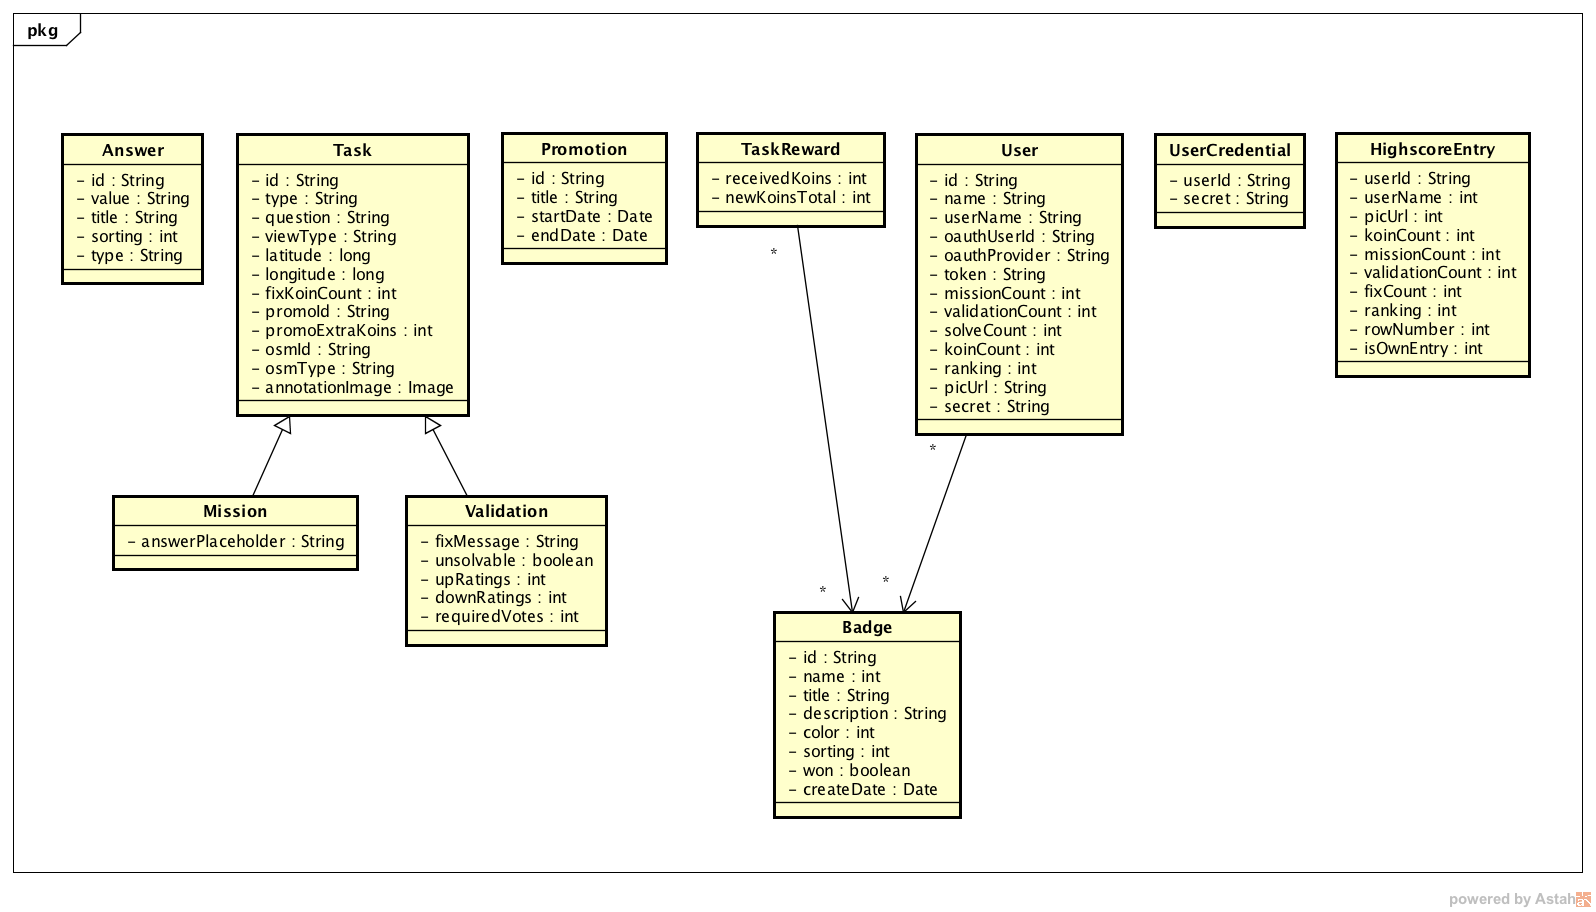
\includegraphics[width=\textwidth]{images/projektdokumentation/Datenmodell.png}
 	\caption{Modellierung der DTOs}
 	\label{image-data-model}
\end{figure}


% Architektur
\label{pd-architektur}
\section{Architektur}
Für unsere Applikationsarchitektur haben wir das \brand{Flux}\footnote{\url{https://facebook.github.io/flux/}} Architekturpattern von \brand{Facebook} eingesetzt.\newline
Die folgenden Erklärungen wurden zu grossen Teilen aus der \brand{Flux} Dokumentation\cite{flux-docs-overview} abgeleitet.
Zu den nachfolgend beschriebenen Konzepten der \brand{Flux}-Architektur mussten für unsere Realisierung keine Anpassungen gemacht werden.
Die Beschreibungen entsprechen also unserer Implementation.\newline
\brand{Flux} ist eine Architektur, die in \gls{Frontend}-Applikationen eingesetzt wird.
Ein unidirektionaler Datenfluss ist das Grundprinzip, auf welchem \brand{Flux} aufbaut, und in welchem es sich von \gls{MVC}-Architekturen unterscheidet.
Das Pattern beschreibt folgende vier Hauptbestandteile: die Stores, die Views (oder Controller-Views), die Actions und der Dispatcher. 
Ein Beispiel, wie die Architektur in der Abbildung ~\ref{image-flux-overview-simple} umgesetzt wurde, ist im Sequenzdiagramm zum \hyperref[pd-sequenzdiagramme-mission]{Lösen einer Mission} beschrieben. 

\begin{figure}[H]
 	\centering
 	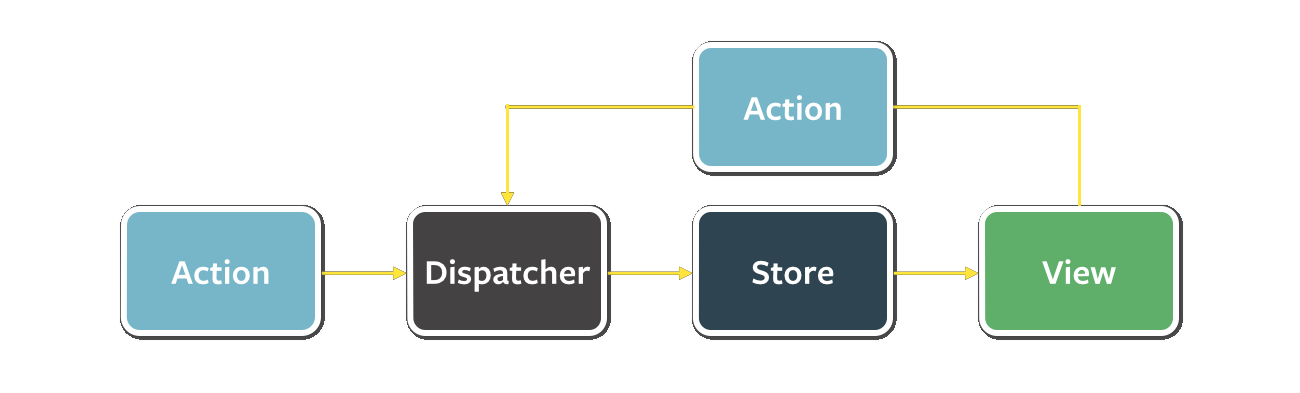
\includegraphics[width=\textwidth]{images/projektdokumentation/flux-uebersicht-weiss.png}
 	\caption{Idee der \brand{Flux}-Architektur}
 	\label{image-flux-overview-simple}
\end{figure}

\subsection{Stores}
\label{pd-flux-stores}
Stores enthalten den Applikationszustand und die Applikationslogik.
Verglichen mit dem \gls{MVC}-Pattern entsprechen sie am ehesten dem Model.
Sie unterscheiden sich aber insofern, dass sie nicht unbedingt einzelne Modellklassen repräsentieren sollen, sondern domänenspezifische Aufgaben übernehmen.
Da \kort{} keine besonders komplexe Domäne enthält, ist diese Unterscheidung allerdings nicht von grosser Bedeutung.
Ein Beispiel für diese Einteilung nach Domäne und nicht nach Modell ist in der Aufteilung von \inlinecode{UserStore} und \inlinecode{AuthenticationStore} zu finden. 
Stores sind als \glslink{Singleton}{Singletons} umgesetzt. 
Sie registrieren sich beim Dispatcher um Updates zu erhalten und ihren Zustand entsprechend anzupassen.
Views wiederum können sich bei den Stores registrieren um neue Informationen zu erhalten, können die Stores aber nicht direkt anweisen, sich zu aktualisieren.

\subsection{Views}
\label{pd-flux-views}
Der Applikationsanwender kommuniziert seine Absichten über die View.
Deshalb gilt die View in \brand{Flux} als Auslöser für neue Aktionen.
In \brand{React} kann zwischen \emph{Views} und \emph{Controller-Views} unterschieden werden.\newline
\emph{Controller-Views} finden sich an der Spitze der View-Hierarchie.
Sie warten auf Updates der Stores und reichen die Daten entlang der Kette ihrer untergeordneten \emph{Views} weiter.\newline
Diese untergeordneten \emph{Views} wiederum reagieren auf Zustandsänderungen indem ihre \inlinecode{render()} Methode neu aufgerufen wird.
Somit bleiben \emph{View} Komponenten modular austauschbar, da sie unabhängig von ihrem Kontext eingesetzt werden können.

\subsection{Actions}
\label{pd-flux-actions}
Actions sind Helfermethoden, welche im Dispatcher ein Ereignis und somit in den Stores ein Update auslösen.
Sie werden ausschliesslich durch Views ausgelöst, da diese für den Kontrollmechanismus der Applikation zuständig sind.
Ausnahmen wären hier denkbar, waren aber nicht nötig.
Beispielsweise könnte der \inlinecode{LocationStore} eine Action auslösen wenn er eine neue Position erkannt hat oder der Server wenn ein Update an die Applikation gesendet werden soll.\newline
Ausserdem sollten Daten, wenn diese für ein Update nötig sind, bereits durch die Actions an den Dispatcher mitgeliefert werden.
Aufrufe an die \gls{REST}-Schnittstelle des \glslink{Backend}{Backends} werden also über die Actions ausgelöst.
Somit kann sichergestellt werden, dass verschiedene Stores, welche auf dieselbe Action reagieren, denselben \gls{API}-Aufruf mehrmals ausführen.
In Abbildung \ref{image-flux-overview-detailed} ist dies ersichtlich.

\subsection{Dispatcher}
\label{pd-flux-dispatcher}
Der Dispatcher ist der zentrale Knotenpunkt, durch den der gesamte Datenfluss der Applikation koordiniert wird.
Seine einzige Aufgabe ist die Verteilung der Actions an die Stores.
Er enthält also keine intelligente Logik, sondern ist grundsätzlich ein Register von Callbacks.\newline
\begin{figure}[H]
 	\centering
 	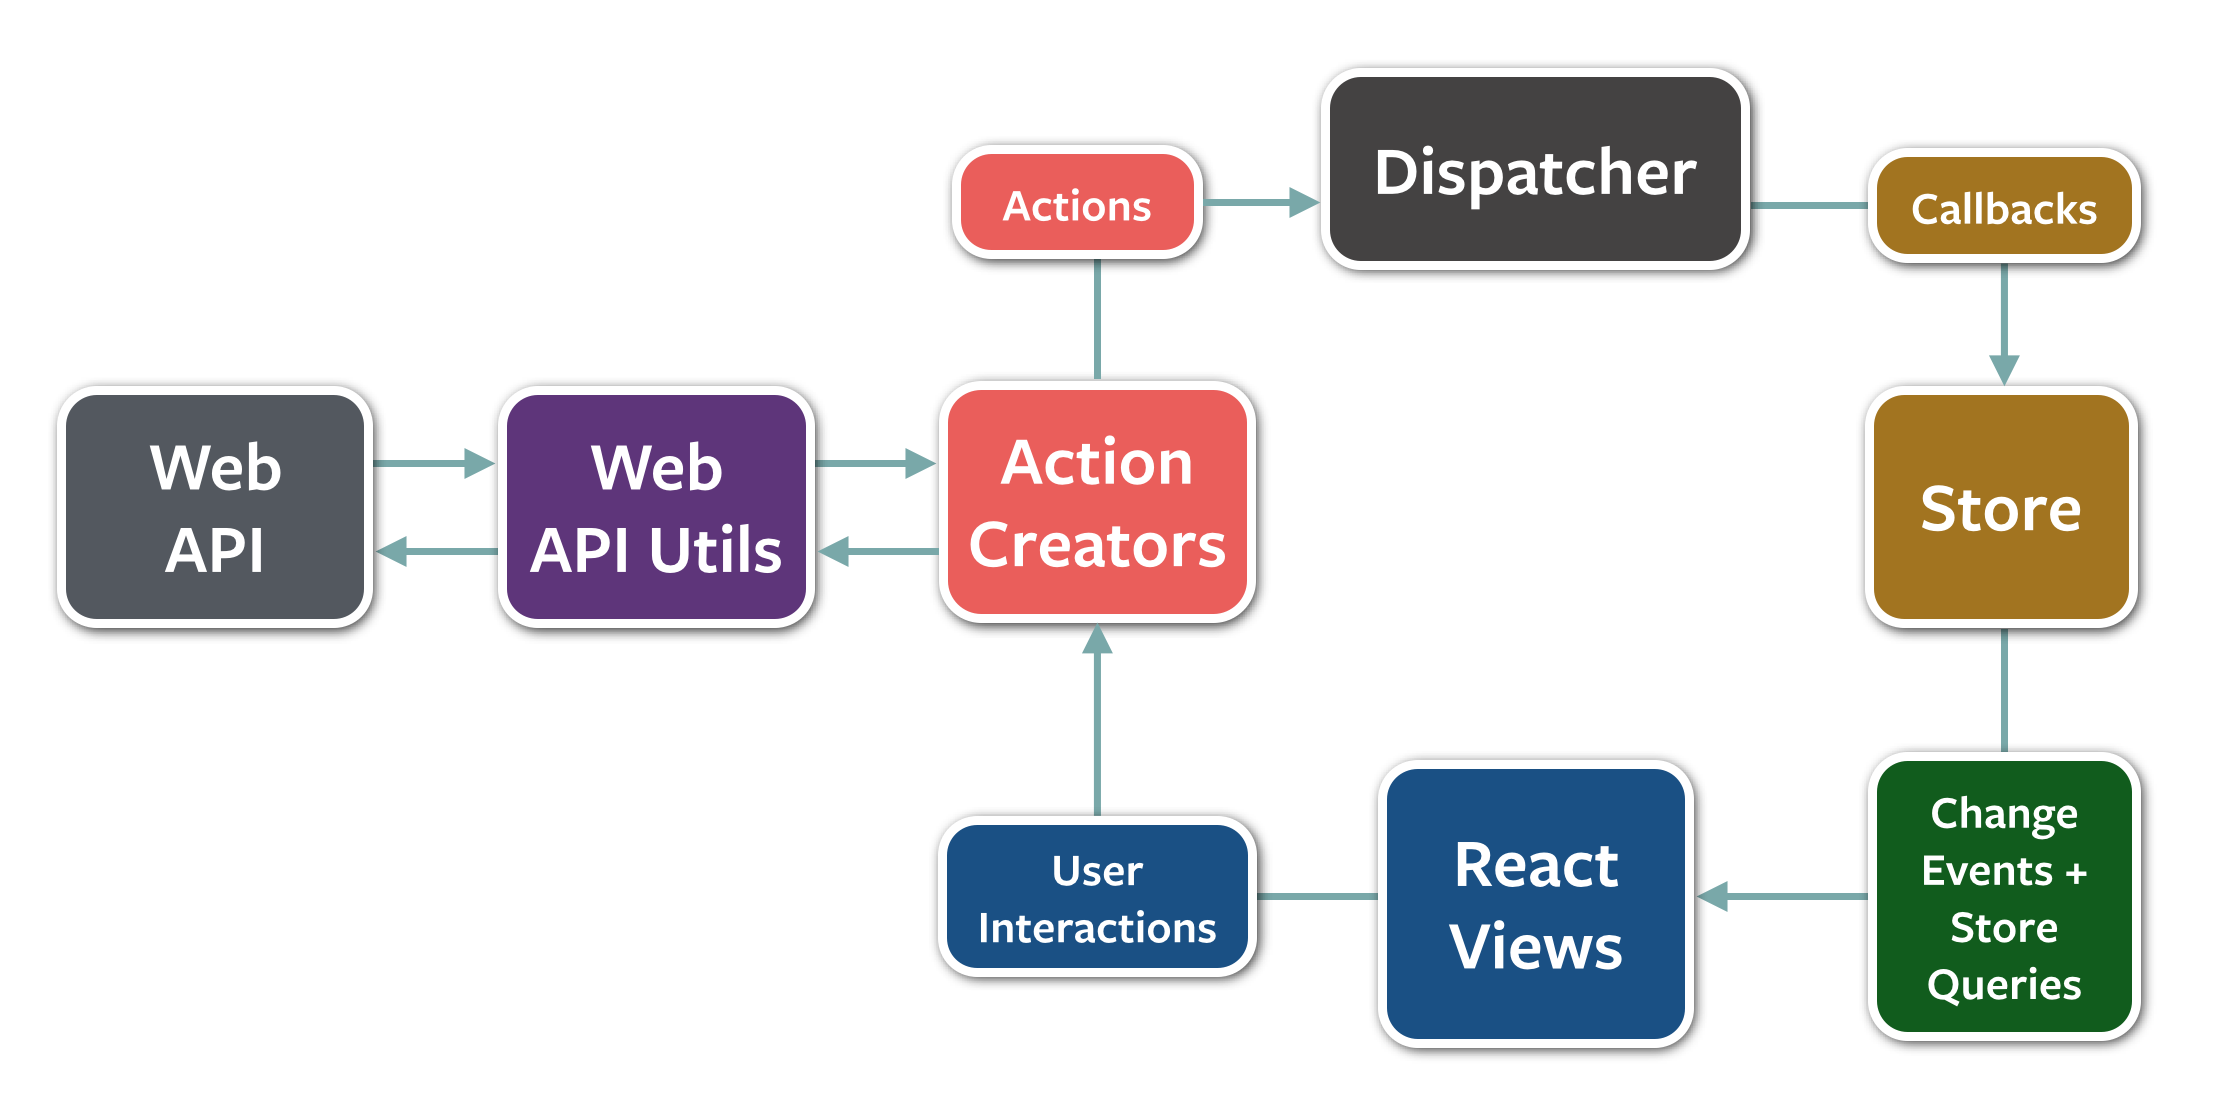
\includegraphics[width=\textwidth]{images/projektdokumentation/flux-diagram.png}
 	\caption{Vollständiges \brand{Flux}-Diagramm\cite{flux-npm-package}}
 	\label{image-flux-overview-detailed}
\end{figure}	

% Sequenzdiagramme
\label{pd-sequenzdiagramme}
\section{Sequenzdiagramme}
\subsection{Starten der App}
\begin{figure}[H]
 	\centering
 	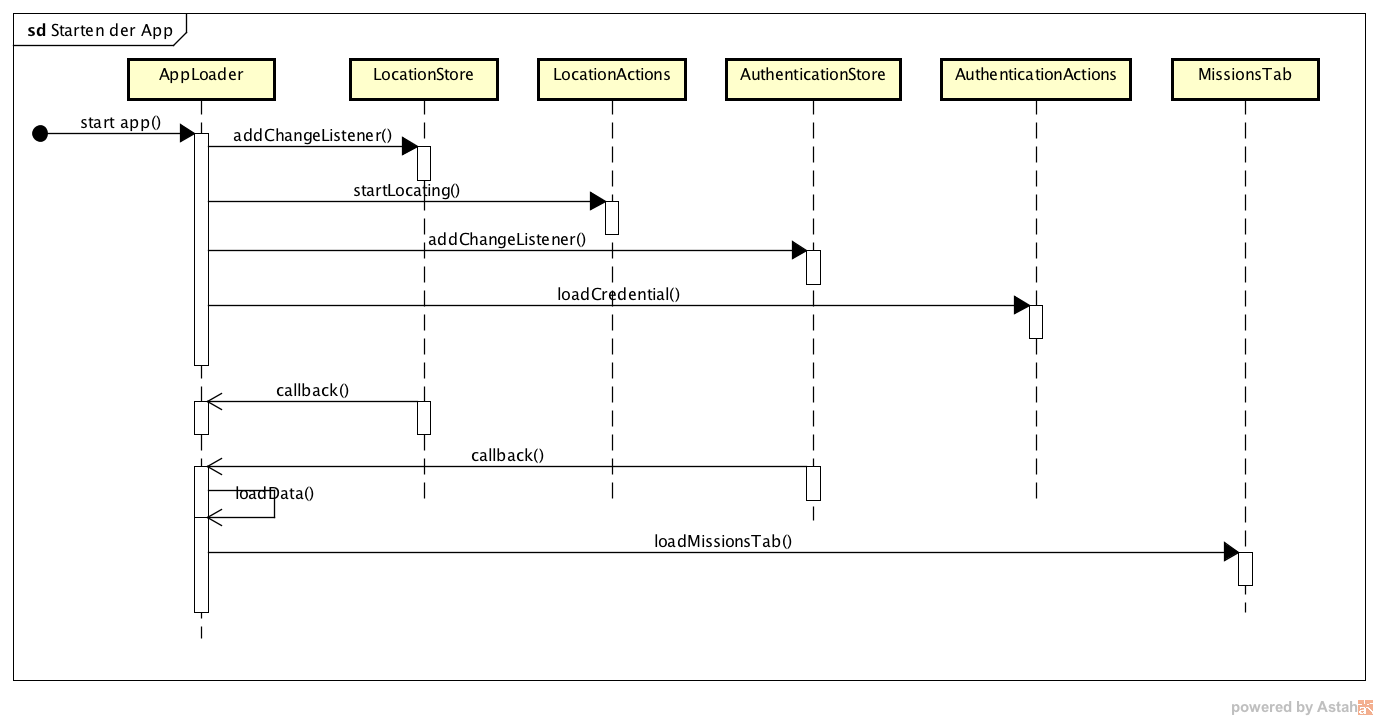
\includegraphics[width=\textwidth]{images/projektdokumentation/sd-app-start.png}
 	\caption{Bevor Daten geladen und Informationen dargestellt werden können, muss der Benutzer autorisiert und lokalisiert sein.}
 	\label{image-sd-start-app}
\end{figure}

\subsection{Mission lösen}
\label{pd-sequenzdiagramme-mission}
\begin{figure}[H]
 	\centering
 	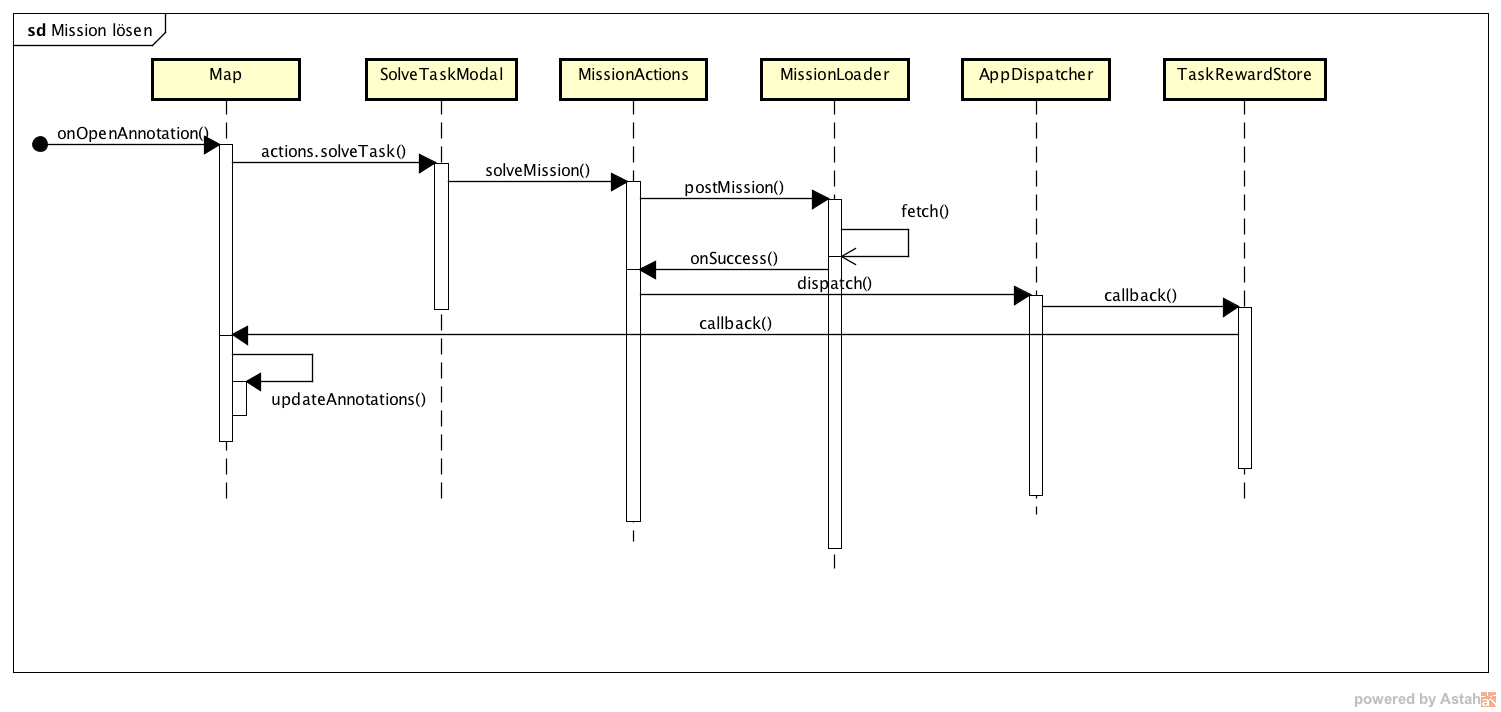
\includegraphics[width=\textwidth]{images/projektdokumentation/sd-mission-loesen.png}
 	\caption{Lösen einer Mission und Anzeigen der Belohnung}
 	\label{image-sd-solve-mission}
\end{figure}

% Entwicklungsumgebung
\chapter{Entwicklungsumgebung}
\label{pd-entwicklungsumgebung}
\section{IDE}
Die Funktionalitäten und Features der App wurden alle mit \brand{Atom} implementiert. 
Für das Debugging waren die native \glslink{IDE}{IDEs} \brand{Android Studio} und \brand{Xcode} aber besser geeignet. 
Das Debuggen in der \brand{Atom}-\gls{IDE} oder im \brand{Google Chrome} Browser war oft fehlerhaft. 
Ansonsten wurden die native \glslink{IDE}{IDEs} nur für das Einfügen von statischen Bildern mit passenden Auflösungen für entsprechende Displays genutzt. 


\section{Continuous Integration}
Als Versionsverwaltungssystem wurde \brand{git}\footnote{\url{https://git-scm.com/}} zusammen mit dem Online-Dienst \brand{GitHub}\footnote{\url{https://github.com}} verwendet: \url{https://github.com/kort/kort-reloaded}.
Dabei haben wir folgendes Branching Model eingesetzt: Der master Branch wird nur für Releases verwendet.
Für die Entwicklung wurde der develop Branch genutzt, wobei jedes Feature und jeder Fix eines Bugs einen eigenen Branch erhielt, welcher nach Fertigstellung wieder in den develop Branch gemerged wurde.\newline
\newline
Für die \gls{CI} (CI) nutzen wir den freien Dienst von \brand{Travis-CI}\footnote{\url{https://travis-ci.org/}}.
Dieses Setup lässt sich bequem in Verbindung mit \brand{GitHub} nutzen. 
Dabei wird bei jeder Neuerung auf dem master und develop Branch über \brand{Travis-CI} ein neuer Build erstellt.
Bei jedem Build werden die Tests durchlaufen und der Code auf die Einhaltung der \nameref{pd-entwicklungsumgebung-cr} überprüft.\newline
Die Konfigurationsdatei für \brand{Travis-CI} (\inlinecode{.travis.yml}) befindet sich im \brand{GitHub}-Repository von \kort{}.

\section{Projektmanagement-Tool}
Als Projektmanagement-Tool wurde \brand{Redmine} verwendet. 
Weiterführende Links zum Redmine-Projekt, das für die Ticketerfassung verwendet wurde, sind im Kapitel \hyperref[pm-projektmanagement]{Projektmanagement} dokumentiert.


\section{Testing}
\label{pd-entwicklungsumgebung-testing}
Fürs Testing wurden \glslink{Unit Test}{Unit Tests}, \glslink{Integration Test}{Integration Tests} und \glslink{Funktionaler Test}{Funktionalen Tests} evaluiert.
Letztlich konnten -- zum Zeitpunkt der Abgabe -- lediglich die Unit Tests umgesetzt werden.
Integration Tests wären für die \inlinecode{data} Klassen wünschenswert gewesen, konnten aber aus Zeitgründen nicht umgesetzt werden.
Automated UI Tests sind mit \brand{React Native} möglich\footnote{Einen guten Überblick bietet diese Seite: \url{http://testdroid.com/tech/testing-react-native-apps-on-android-and-ios}}, sind aber sehr aufwendig einzurichten.
Für die Unit Tests wurde \brand{Jest}\footnote{\url{https://facebook.github.io/jest/}} eingesetzt. 
\brand{Jest} ist ein \brand{JavaScript} Testing-\gls{Framework} und wird zum Beispiel von \brand{Facebook} zum Testen von \brand{React}-Applikationen verwendet.\newline
Eine besondere Eigenschaft von \brand{Jest} ist, dass standardmässig für alle Module automatisch \glslink{Mock}{Mocks} bereitgestellt werden.
Somit wird verhindert, dass aus Versehen das Verhalten anderer Module getestet wird.

\section{Code-Richtlinien}
\label{pd-entwicklungsumgebung-cr}
Um Code-Richtlinien festzulegen und deren Einhaltung zu prüfen, wurde \brand{ESLint}\footnote{\url{http://eslint.org/}} eingesetzt.
Dadurch wird die die Lesbarkeit und Wartbarkeit des Codes erhöht.
Die Konfiguration von \brand{ESLint} stammt von \brand{Airbnb}\footnote{\url{https://github.com/airbnb/javascript/tree/master/packages/eslint-config-airbnb}}.
Darüber hinaus wurden Plugins für \brand{React}\footnote{\url{https://github.com/yannickcr/eslint-plugin-react}} und \brand{React Native}\footnote{\url{https://github.com/Intellicode/eslint-plugin-react-native}} eingesetzt.\newline
Die Konfiguration findet sich in der Datei \inlinecode{.eslintrc.json}.

% Implementation
\chapter{Implementation}
\label{pd-implementation}
Dieses Kapitel beschreibt die Einrichtung und Implementation von den folgenden \glslink{Library}{Libraries} und Komponenten. 
Beim Entwickeln der \brand{Android}-App wurde darauf geachtet, dass möglichst keine Plattform spezifische Komponenten zu nutzen. 
Das konnte in diesem Projekt erfolgreich umgesetzt werden. 
Die einzige spezifische Komponente ist der Ladebildschirm, der jeweils auch für die \brand{iOS}-Version erstellt wurde.
Aus Zeitgründen konnte die \brand{iOS}-Version aber nicht getestet werden. 


\section{Kort Backend}
Das \kort{}-Backend existierte bereits und wurde von den Entwicklern nicht mehr abgeändert. 
Es ist im Kapitel 10.2. \gls{REST}-Schnittstellen der Bachelorarbeit von Jürg Hunziker und Stefan Oderbolz dokumentiert.\cite{ba-kort-2012}

\section{View Components}
\label{pd-implementation-components}
Components entsprechen den \hyperref[pd-flux-views]{Views} der \brand{Flux}-Architektur.
Component Klassen erweitern \inlinecode{React.Component}\footnote{\url{https://facebook.github.io/react/docs/component-api.html}} und implementieren mindestens die \inlinecode{render()} Methode\footnote{\url{https://facebook.github.io/react/docs/component-specs.html}}. 
In der \inlinecode{render()} Methode wird in \gls{JSX} Syntax definiert, wie die Component dargestellt werden soll.\newline
Eine Component kann andere Components wiederverwenden,
Dadurch wird sowohl ein hierarchischer Aufbau der View, als auch ein modularer Einsatz von Components  ermöglicht.\newline
Ein weiteres Konzept, das von Components realisiert wird, ist die Unterscheidung von Property und State.
Eine Property repräsentiert eine sich nicht ändernde Eigenschaft einer Component, während der State den aktuellen Zustand ausdrückt.
Properties werden vom Owner\footnote{Die Owner-Ownee-Beziehung wird unter \emph{Ownership} beschrieben: \url{https://facebook.github.io/react/docs/multiple-components.html}} gesetzt und können durch den Ownee als \inlinecode{propTypes} deklariert werden.
Wird eine State Variable neu gesetzt, führt dies zu einem erneuten Aufruf der \inlinecode{render()} Methode.\newline
Components dürfen den Zustand -- der in den Stores gehalten wird -- nie direkt manipulieren, sondern müssen dies über Actions auslösen.
In den Callbacks, welche sie bei den Stores registriert haben, können sie dann die Getter aufrufen um den neuen Zustand zu erhalten.
Components sollen nicht mehr über den Applikationszustand wissen als für ihre Ansicht nötig ist.
Die Logik sollte also so weit möglich in den Stores umgesetzt sein.\newline

\section{Libraries}
Damit die entsprechenden \glslink{Library}{Libraries} genutzt werden können, mussten sie mit dem Node-Package-Manager (npm) heruntergeladen werden. 
Mit dem \inlinecode{npm install}-Befehl wurden alle aufgelisteten Abhängigkeiten in der  \inlinecode{package.json}-Datei installiert und im Ordner \newline\inlinecode{node-modules} gespeichert.
Wenn eine Library eine Bridge zu nativem Code verwendet, muss sie zusätzlich im \brand{Android}- und \brand{iOS}-Projekt gelinkt werden. 
Dann konnten die Libraries in einer \brand{JavaScript}-Komponente importiert und verwendet werden.

\begin{table}[H]
\centering
\begin{tabular}{|p{0.25\threecelltabwidth}|p{0.15\threecelltabwidth}|p{0.60\threecelltabwidth}|}
\hline 
\textbf{Library} & \textbf{Version} & \textbf{Verwendung} \\
\hline 
flux & 2.1.1 & Nutzung des \hyperref[pd-flux-dispatcher]{Dispatchers} \\
\hline 
react & 15.0.2. & Entwicklung vom User Interface \\
\hline 
react-native & 0.26.3 & Entwicklung von native Apps mit \brand{React} \\
\hline 
react-native-google-signin & 0.6.0 & Native Authentifizierung mit Google OAuth \\
\hline 
react-native-i18n & 0.0.8 & Internationalisierung der Benutzeroberfläche \\
\hline 
react-native-mapbox-gl & 4.1.1 & Darstellung der Karte \\
\hline 
react-native-router-flux & 3.26.15 & Navigation im User Interface \\
\hline 
\end{tabular}
\caption{Abhängigkeiten im \brand{JavaScript}-Code}
\label{table-dependencies}
\end{table}

\begin{table}[H]
\centering
\begin{tabular}{|p{0.25\threecelltabwidth}|p{0.15\threecelltabwidth}|p{0.60\threecelltabwidth}|}
\hline 
\textbf{Library} & \textbf{Version} & \textbf{Verwendung} \\
\hline 
babel-eslint \newline
babel-jest \newline
babel-polyfill \newline
babel-preset-es2015 \newline
babel-preset-react \newline
babel-preset-react-native-stage-0
& 
6.0.4 \newline
12.1.0 \newline
6.9.0 \newline
6.6.0 \newline
6.5.0 \newline
1.0.1
& Compiler für die verschiedenen Libraries und \brand{ES2015} \\
\hline 
eslint \newline
eslint-config-airbnb \newline
eslint-plugin-react \newline
eslint-plugin-react-native
&
2.11.1 \newline
6.2.0 \newline
4.3.0 \newline
1.0.0
& Einhaltung der \nameref{pd-entwicklungsumgebung-cr} \\
\hline 
jest & 12.1.1 & \nameref{pd-entwicklungsumgebung-testing} \\
\hline 
\end{tabular}
\caption{Abhängigkeiten für die Entwicklung}
\label{table-dev-dependencies}
\end{table}

Die vollständige Übersicht aller Abhängigkeiten finden sich in der Datei \inlinecode{package.json}.

\subsection{Navigation}
Die Implementation der Navigation wurde in der Einstiegs-Komponente der App umgesetzt. 
Alle Scenes werden mit einem Key deklariert und falls nötig mit Optionen für eine Tab-Ansicht erweitert. 
Die definierten Scenes werden als Kind-Komponenten einem Router übergeben. 
Jede Scene kann mit einem Funktionsaufruf 
\begin{itemize}
	\item die Properties aktualisieren.
	\item sich selber schliessen.
	\item eine andere Scene mit dem Key und mit optionalen Properties, als Parameter, aufrufen.
\end{itemize} 
Die \gls{API} der Navigations-Komponente ist auf der entsprechenden \brand{GitHub}-Seite\footnote{\url{https://github.com/aksonov/react-native-router-flux}} dokumentiert. 


\subsection{Karte}
Um die Map-Komponente von \brand{Mapbox} zu nutzen und ein Access-Token zu erhalten, muss auf der \brand{Mapbox}-Webseite\footnote{\url{https://www.mapbox.com/}} ein Benutzerkonto angelegt werden. 

Damit die Marker an der richtigen Position angezeigt werden, wurden der \brand{Mapbox}-Komponente ein Array mit Annotations als Parameter übergeben. 
Das Annotation-Array wird fortlaufend mit allen Missionen vom \gls{Backend} aktualisiert. 
Dabei werden nur Missionen in der Umgebung des Benutzers geladen. 
Eine Annotation enthält die Koordinaten und die ID einer Mission. 
Es war von der \brand{Mapbox}-\gls{API} her nicht möglich, einer Annotation direkt die Mission als Objekt mitzugeben. 
Bei einem Klick auf einen Marker wird die Funktion \inlinecode{onOpenAnnotation} aufgerufen.
Diese Funktion öffnet wiederum eine Scene, die es dem Benutzer erlaubt, die gewählte Mission zu lösen.
Die \brand{Mapbox}-\gls{API} ist auf der entsprechenden \brand{Github}-Seite\footnote{\url{https://github.com/mapbox/react-native-mapbox-gl}} dokumentiert. 


\subsection{OAuth}
Für die Authentifizierung über \brand{Google} wurde eine Open Source \gls{Library} evaluiert (Kapitel Evaluation \nameref{tb-evaluation-oauth}). 
Damit die App sich mit der \brand{Google}-\gls{API} verbinden kann, muss eine \inlinecode{google-services.json}-Datei auf der \brand{Google}-Webseite\footnote{\url{https://developers.google.com/cloud-messaging/android/client}} generiert werden. 
Diese Datei enthält die Konfiguration des \brand{Google}-Developer Kontos. 

Nach dem Login des Benutzers erhält die App über diese \gls{Library} das Benutzer-Token von \brand{Google}.
Dieses Token wird dann von der App dem \kort{}-\gls{Backend} mitgeteilt und von dort aus bei \brand{Google} überprüft. 
Wie die Authentifizierung auf der \gls{Backend}-Seite weiter verläuft ist im Kapitel 10.4.1. der Bachelorarbeit von Jürg Hunziker und Stefan Oderbolz beschrieben.\cite{ba-kort-2012}

% Weiterentwicklung
\chapter{Weiterentwicklung}
\label{pd-weiterentwicklung}

\kort{} hat grosses Potenzial um weiterentwickelt zu werden.
Dieses umfasst vor allem zwei Bereiche:

\begin{itemize}
	\item Wie kann \kort{} besser dazu beitragen, \brand{OSM} Daten zu verbessern?
	\item Und wie kann der Benutzer mithilfe von Konzepten der Gamification weiter motiviert werden, zur Datenpflege beizutragen?
\end{itemize}

Wir haben uns Gedanken dazu gemacht und hier zusammengefasst, wie \kort{} weiter optimiert werden könnte.
Das Unterkapitel \hyperref[pd-weiterentwicklung-vorgehen]{Vorgehen} enthält Arbeiten, die beim derzeitigen Stand noch verbessert werden müssen. 
Weiterhin sind Ideen aufgelistet, die keine grösseren Änderungen am Backend mit sich bringen.

\section{Vorgehen}
\label{pd-weiterentwicklung-vorgehen}
Ein sehr wichtiges Feature, das bisher noch nicht umsetzbar war, ist der \brand{OSM}-Login.
Neben den Änderungen am Backend (damit dieses Feature überhaupt brauchbar ist) gibt es folgende Schritte zu erledigen:

\begin{enumerate}
	\item App bei \brand{OSM} mit Callback-URL registrieren
	\begin{itemize}
		\item Als Callback-URL könnte zum Beispiel 'http://www.kort.ch/' verwendet werden.
	\end{itemize}
	\item \brand{OSM}-Request-Token-URL aufrufen um das OAuth-Token und das Token-Secret zu erhalten
	\item \brand{OSM}-Authorize-URL mit dem OAuth-Token aufrufen, damit sich der Benutzer auf der \brand{OSM}-Seite einloggen kann
	\item WebView-Component öffnen um auf die Callback-URL zu warten 
	\item Wenn sich der Benutzer eingeloggt hat, wird er zur Callback-Seite mit dem OAuth-Token und dem OAuth-Verifier in der URL umgeleitet.
	\item WebView schliessen
	\item Request \brand{OSM}-Access-Token-URL
	\item Dem Backend das Token zur Überprüfung senden
\end{enumerate}

Dieses Vorgehen wurde noch nicht getestet und dient nur als Idee zur möglichen Umsetzung.
Die korrekten Request-URLs können aus der Dokumentation im \brand{OSM}-Wiki\footnote{\url{http://wiki.openstreetmap.org/wiki/OAuth}} entnommen werden.

Als Nächstes müsste für den \gls{Gamification}-Ansatz das Design weiter verbessert werden. 
Dafür wäre zuerst eine Änderung am Backend geplant um die Validierungen endgültig abzuschaffen, indem sie als normale Missionen gezählt werden. 
Dann wäre es auch wieder möglich, korrekte Badges für den Missionen-Counter anzuzeigen. 

Durch den Einsatz von Farben oder einem Hintergrundbild beim Login-Screen würde das Design einen Spieler besser ansprechen. 
Passend dazu könnten die verwendeten Bilder, Icons und Marker einheitlich gestaltet und erneuert werden. 

Meldungen, die dem Benutzer die Anzahl gewonnener Koins anzeigen, erscheinen momentan im Vollbildmodus. 
Das liegt an einem Fehler der eingesetzten Navigations-Komponente, die keine transparenten Hintergründe zulässt. 
In Zukunft könnte das aber noch behoben werden. 
Dann wäre es eleganter, Meldungen in einem Fenster zu zeigen.

\subsubsection{GUI-Arbeiten}
\begin{itemize}
	\item Alle Map-Marker ersetzen.
	\item Textfeld zur Anpassung des Benutzernamens anbieten.
	\item Layout und Design aufbessern.
	\item Tab-Icons für \brand{iOS} einfügen.
\end{itemize}

Bis die Funktionalität der \gls{WebApp} komplett umgesetzt ist, fehlen noch zwei Features. 
Diese wären die zweite Highscore-Ansicht und die Karte, die beim Lösen einer Mission angezeigt wird. 
Die zweite Highscore-Ansicht zeigt den eingeloggten Benutzer mit seinen direkten Konkurrenten, die vor und nach ihm platziert sind. 
Wenn sich der Benutzer in der Ansicht zum Lösen einer Mission befindet, gäbe es in einem weiteren Tab eine Karte, die das Objekt der Mission hervorgehoben anzeigt. 

Gerne hätten wir noch Tests der \inlinecode{Components} durchgeführt, doch die Priorität dafür war zu tief und die Zeit zu knapp. 
Dazu haben wir für die Zukunft die Enzyme\footnote{\url{http://airbnb.io/enzyme/}}-Testing-API (für \inlinecode{Component}-Tests) und das Mocha\footnote{\url{https://github.com/mochajs/mocha}}-\gls{Framework} (um die Tests laufen zu lassen) evaluiert.

\section{Weiterführende Arbeiten}
\label{pd-weiterentwicklung-realistisch}
Punkte, die \kort{} attraktiver machen würden:

\begin{itemize}
	\item Benutzerlogin mit weiteren \gls{OAuth}-Diensten erweitern (z.\,B. \brand{Twitter}, \brand{GitHub})
	\item \gls{Gamification}
	\begin{itemize}
		\item Von gesammelten \emph{Koins} abhängige Levels einführen (z.\,B. bestimmte Fehlertypen erst ab fortgeschrittenem Level anzeigen, Avatars, Levelbezeichnungen)
		\item Verschiedene Schwierigkeitsstufen
		\item Einbindung in \brand{Game Center} der jeweiligen Plattform
		\item Weitere Badges einführen (viele Ideen finden sich hier: \url{https://wiki.openstreetmap.org/wiki/Badges}, z.\,B. auch Badges für Spielertypen)
		\item Verschiedene Highscores anzeigen (z.\,B. zeitlich oder Regional begrenzt, nach Fehlertypen kategorisiert, schnellste Aufsteiger)
		\item Zusätzliche Berechtigungen für erfahrene Benutzer (für den langfristigen Erfolg)
	\end{itemize}
	\item Neue realistische Fehlertypen\footnote{\url{https://github.com/kort/kort/issues/81}}
	\begin{itemize}
		\item Hausnummern einfügen
		\item Stockwerk-Anzahl einfügen
		\item Einbahnstrassen erfassen
		\item Öffnungszeiten von öffentlichen Gebäuden festhalten
	\end{itemize}
	\item Weniger realistische Fehlertypen
		\begin{itemize}
			\item Kreisel erfassen
			\item Bushaltestellen von \brand{DIDOK}\footnote{\url{https://didok.osm.ch/}} erfassen
		\end{itemize}
	\item Erkennen von Benutzern, die nicht sorgfältig validieren\footnote{\url{https://github.com/kort/kort/issues/7}}
	\item Ausführliche Statistiken für individuelle Benutzer\footnote{\url{https://github.com/kort/kort/issues/71}}
	\item Aufträge aus \brand{wheelmap}\footnote{\url{http://wheelmap.org}}	einfügen
	\item Offline-Fähigkeit (offline Maps für \brand{React Native} wären erforderlich)
	\item Wenn Aufträge z.\,B. drei Mal nicht gelöst werden können, soll eine \brand{OSM}-Notiz generiert werden
\end{itemize}

\subsubsection{Unrealistische Arbeiten}
Folgende Punkte wurden in einem Meeting mit den Entwicklern und dem Betreuer (Prof. Stefan Keller) besprochen. 
Sie sind für \kort{} als weniger geeignet empfunden worden.

\begin{itemize}
	\item Erweitern der Verifizierung mit der Möglichkeit, ein Foto als Beweis hochzuladen
	\begin{itemize}
	  \item \emph{Begründung:} Aspekte des Datenschutzes bergen ein gewisses Risiko. Benutzer müssten für das Hochladen von Bildern zusätzliche Bedingungen akzeptieren.
	\end{itemize}
	\item standortunabhängige Aufgaben lösen (Gefahr von Couch Mapping)
	\begin{itemize}
	  \item \emph{Begründung:} Es ist ein Anliegen der \brand{OSM} Community, dass die Mapper vor Ort sein sollen um Aufträge zu lösen. 
	\end{itemize}
\end{itemize}


% Installation
\chapter{Installation}
\label{pd-installation}

In diesem Kapitel werden zwei Varianten beschrieben, wie die App getestet werden kann. 


\section{Installation mit Source Code}
Um die App anhand des Source Codes zu installieren, muss die \brand{React Native} Entwicklungsumgebung aufgesetzt sein. 
Wie diese eingerichtet wird, ist in der Getting-Started-Anleitung, der Onlinedokumentation von \brand{React Native}\footnote{\url{https://facebook.github.io/react-native/docs/getting-started.html}}, erklärt.
Diese Anleitung erklärt Schritt für Schritt den Ablauf von der Einrichtung der Entwicklungsumgebung auf einem \brand{Mac}-, \brand{Linux}- oder \brand{Windows}-Rechner (für \brand{iOS} und \brand{Android}) bis zum Starten der App.

Hier muss noch beachtet werden, dass die SecretConfig.js-Datei mit folgenden Werten ergänzt werden sollte.
Der Dateipfad lautet: \inlinecode{/kort-reloaded/js/constants/SecretConfig.js}\newline

\begin{itemize}
	\item Mapbox Access Token
	\begin{itemize}
		\item Dieses Token kann auf der Mapbox-Webseite\footnote{\url{https://www.mapbox.com/help/create-api-access-token/}} erstellt werden.
	\end{itemize}
	
	\item Google Client ID 
	\begin{itemize}
		\item Wie die Google Client ID erhalten wird, ist in der Anleitung des \brand{GitHub}-Projekts der Google-Signin-Library erklärt.\footnote{\url{https://www.mapbox.com/help/create-api-access-token/}}
		\item Wichtig ist, dass anhand dieser Anleitung auch die google-services.json-Datei neu generiert und in das Projekt eingefügt werden muss.
	\end{itemize}
\end{itemize}

\section{Installation mit APK-Datei}
Damit die \brand{Android}-App von der bereitgestellten APK-Datei auf der CD installiert werden kann, muss das Smartphone mit dem Computer per USB-Kabel verbunden sein und erkannt werden. 

\begin{enumerate}
	\item Die APK-Datei in einen Ordner auf dem Gerätespeicher kopieren.
	\item Die Smartphone Verbindung mit dem Computer trennen.
	\item Die APK-Datei auf dem Smartphone auffinden und anklicken.
	\item Dem App-Herausgeber vertrauen und Installation abschliessen.
\end{enumerate}


% Neue Seite beginnen
\cleardoublepage

% Projektmanagement
\part{Projektmanagement}
%Projektmanagement
\chapter{Projektmanagement}
\label{pm-projektmanagement}
Hier sind die Angaben zum Projekt, zu den eingesetzten Entwicklungswerkzeugen und zur eingesetzten Software zu finden.

\begin{itemize}
    \item Website: \url{http://www.kort.ch/} (\url{http://play.kort.ch/})
    \item Source Code: \url{https://github.com/kort/kort-reloaded/}
    \item Dokumentation: \url{https://github.com/kort/kort-reloaded-docu}
    \item Projektmanagement: Redmine (\url{sinv-56059.edu.hsr.ch/redmine/projects/ba-kort/ })
    \item Issues: \url{http://sinv-56059.edu.hsr.ch/redmine/projects/ba-kort/issues}  (Backlog: im Wiki auf Redmine) 
\end{itemize}

\section{Team}
\label{pm-team}
\begin{itemize}
	\item \textit{Betreuer}: Prof. Stefan F. Keller
	\item \textit{Projektpartner}: Liip AG, Limmatstrasse 183, CH-8005 Zürich
	\begin{itemize}
		\item Jürg Hunziker
		\item Stefan Oderbolz
	\end{itemize}
	\item \textit{Experte}: Claude Eisenhut
	\item \textit{Gegenleser}: Prof. Beat Stettler
\end{itemize}

\subsection*{Autoren}
\label{pm-team-autoren}
Diese Arbeit wird als Bachelorarbeit an der Abteilung Informatik durchgeführt von
\begin{itemize}
	\item Marino Melchiori
	\item Dominic Mülhaupt
\end{itemize}

\subsection*{Aufgabenbereiche}
Jeweils zu Beginn eines Sprints wurden die Zuständigkeiten aufgeteilt, abgearbeitet und am Ende besprochen. 

Einige Kernpunkte der Aufgabenbereiche von Marino Melchiori waren:
\begin{itemize}
	\item \gls{OAuth}
	\item \gls{GUI}
	\item Map
\end{itemize}

Die Aufgabenbereiche von Dominic Mülhaupt waren:
\begin{itemize}
	\item Daten-Layer
	\item Stores
	\item \brand{Flux}
	\item Setup (\brand{GitHub}, \brand{Travis-CI})
\end{itemize}


\section{Risikomanagement}
\label{pm-projektmanagement-risikomanagement}
Da \kort{} bereits in einer vorhergehenden Bachelorarbeit erfolgreich umgesetzt werden konnte und Anklang gefunden hat, wurden bereits viele Risiken abgedeckt.\newline
Dennoch wurde das Risikomanagement nicht vernachlässigt.
Alle bekannten Risiken sind gesammelt aufgelistet und wurden nach jedem Meilenstein neu evaluiert.

\subsection{Risikoanalyse}
\label{pm-projektmanagement-risikoanalyse}
Am Anfang der Bachelorarbeit wurden folgende Risiken identifiziert:

\begin{table}[H]
\centering
\label{pm-projektmanagement-risikomanagement-r01}
\begin{tabular}{|>{\raggedright}p{4.5cm}|p{11cm}|}
\hline
\multicolumn{2}{|l|}{\textbf{R01: Mangelnde Erfahrung mit \brand{JavaScript}, \brand{React} und \brand{React Native}}} \\
\hline
\textbf{Beschreibung} & Wirkt sich negativ auf Design und Programmcode aus. \\
\hline
\textbf{Schadenspotential} & 60h \\
\hline
\textbf{Eintrittswahrsch.} & 65\,\% \\
\hline
\textbf{Auswirkung} & Da die Entwickler sich mit den zugrundeliegenden Programmierkonzepten vertraut machen während sie bereits planen und Entscheidungen treffen, teilweise sogar schon programmieren müssen, kann und wird es vorkommen, dass gewisse Entscheidungen schlecht getroffen und gewisse Konzepte nicht sauber umgesetzt werden. 
Dies kann zu Verspätungen oder unsauberem Programmcode führen. \\
\hline
\textbf{Vorbeugung} & Die Entwickler haben mit dem Betreuer (Prof. Stefan Keller) besprochen, dass das \gls{Minimum Viable Product} der Bachelorarbeit eine Android App mit der gleichen Funktionalität, wie sie bereits im ursprünglichen Kort Game umgesetzt wurde, sein wird.
Im Rahmen dieser Arbeit blieb aber schlicht keine Zeit, um sich umfassend in die Technologien einzuarbeiten, bevor die restliche Arbeit angepackt ist.
Aus diesem Grund wird vor allem zu Beginn vermehrt auf \gls{Pair Programming} gesetzt.
Die Entwickler haben sich auch in regelmässigen Abständen die Zeit genommen, ein Code Review durchzuführen.
Ausserdem ist es wichtig, dass bei Schwierigkeiten nicht zu lange gezögert wird, den Kontakt zu Experten im jeweiligen Bereich zu suchen.  \\
\hline
\textbf{Massnahmen beim Eintreffen} & Komplexe Features vereinfachen und so gestalten, dass sie leicht erweiterbar sind. \\
\hline
\end{tabular}
\caption{Risiko R01}
\end{table}

\begin{table}[H]
\centering
\label{pm-projektmanagement-risikomanagement-r02}
\begin{tabular}{|>{\raggedright}p{4.5cm}|p{11cm}|}
\hline
\multicolumn{2}{|l|}{\textbf{R02: Es existiert keine passende Map Library für \brand{React Native}}} \\
\hline
\textbf{Schadenspotential} & 70h \\
\hline
\textbf{Eintrittswahrsch.} & 30\,\% \\
\hline
\textbf{Auswirkung} & Es müsste statt \brand{React Native} ein alternatives mobiles \gls{Framework} gefunden werden, welches die \brand{OSM}-Daten anzeigen kann. \\
\hline
\textbf{Vorbeugung} & Zu Beginn des Projektes muss eine \brand{React Native} Prototyp-Applikation implementiert werden, welche \brand{OSM}-Daten auf der Karte darstellt.  \\
\hline
\textbf{Massnahmen beim Eintreffen} & Auf eine aufwendigere Variante der Kartendarstellung, die im Kapitel \hyperref[tb-evaluation-karte]{Evaluation} evaluiert wurde, zurückgreifen. \\
\hline
\end{tabular}
\caption{Risiko R02}
\end{table}

\begin{table}[H]
\centering
\label{pm-projektmanagement-risikomanagement-r03}
\begin{tabular}{|>{\raggedright}p{4.5cm}|p{11cm}|}
\hline
\multicolumn{2}{|l|}{\textbf{R03: \brand{KeepRight} stellt den Dienst ein}} \\
\hline
\textbf{Schadenspotential} & 70h \\
\hline
\textbf{Eintrittswahrsch.} & 10\,\% \\
\hline
\textbf{Auswirkung} & Die Anzahl der zur Verfügung stehenden Missionen würde stark eingeschränkt werden.
Ausserdem wären diese auf die Schweiz beschränkt.
Ein anderer Dienst (z.\,B. \brand{Osmose}) müsste eingesetzt werden, was vor allem Änderungen im Backend erfordern würde. \\
\hline
\textbf{Vorbeugung} & Bereits früh im Projekt wird das Thema mit dem \hyperref[pm-team]{Projektpartner} besprochen, um festzustellen, ob dieser bereit wäre, sich dieser Problematik anzunehmen. \\
\hline
\textbf{Massnahmen beim Eintreffen} & Ausarbeitung einer neuen Aufgabenstellung mit dem Betreuer und den Projektpartnern (Jürg Hunziker und Stefan Oderbolz), die Änderungen am Backend beinhaltet. \\
\hline
\end{tabular}
\caption{Risiko R03}
\end{table}

\begin{table}[H]
\centering
\label{pm-projektmanagement-risikomanagement-r04}
\begin{tabular}{|>{\raggedright}p{4.5cm}|p{11cm}|}
\hline
\multicolumn{2}{|l|}{\textbf{R04: \brand{React Native} ist noch nicht ausgereift genug für \brand{Android}}} \\
\hline
\textbf{Schadenspotential} & 20h \\
\hline
\textbf{Eintrittswahrsch.} & 30\,\% \\
\hline
\textbf{Auswirkung} & \brand{Android} wird erst seit Oktober 2015 durch \brand{React Native} unterstützt. 
Einige Features von Komponenten stehen nur für \brand{iOS} zur Verfügung. \\
\hline
\textbf{Vorbeugung} & Bevor mit der Implementation begonnen wurde, sind die mangelnden Funktionalitäten (z.\,B. im Testing), so weit möglich, analysiert.
Grundsätzlich sollte es möglich sein, die App für \brand{Android} umzusetzen, da bereits komplexere Apps damit erstellt wurden.
Wahrscheinlich wird es vorkommen, dass Workarounds nötig sein werden. 
Im schlimmsten Fall müsste während der Entwicklung auf \brand{iOS} umgestellt werden, was grundsätzlich möglich ist. \\
\hline
\textbf{Massnahmen beim Eintreffen} & Ausarbeitung einer neuen Aufgabenstellung mit dem Betreuer, die eine \brand{iOS}-Version bevorzugt. \\
\hline
\end{tabular}
\caption{Risiko R04}
\end{table}

\begin{table}[H]
\centering
\label{pm-projektmanagement-risikomanagement-r05}
\begin{tabular}{|>{\raggedright}p{4.5cm}|p{11cm}|}
\hline
\multicolumn{2}{|l|}{\textbf{R05: Mangelnde Erfahrung mit der flux-Architektur}} \\
\hline
\textbf{Beschreibung} & Wirkt sich negativ auf Design und Programmcode aus. \\
\hline
\textbf{Schadenspotential} & 30h \\
\hline
\textbf{Eintrittswahrsch.} & 40\,\% \\
\hline
\textbf{Auswirkung} & Da die Konzepte der flux-Architektur neu erarbeitet werden müssen und flux in der Community als eher komplex eingestuft wird, kann die Entwicklung mehr Zeit beanspruchen. \\
\hline
\textbf{Vorbeugung} & Die korrekte Umsetzung wird bereits vor dem Start der Implementation so weit wie möglich analysiert.
Dabei wurden die Themengebiete zum Einlesen aufgeteilt und schlussendlich besprochen und erklärt. \\
\hline
\textbf{Massnahmen beim Eintreffen} & Rücksprache mit dem IFS-Team, das an einem \brand{React}-Projekt arbeitet. \\
\hline
\end{tabular}
\caption{Risiko R05}
\end{table}

\begin{table}[H]
\centering
\label{pm-projektmanagement-risikomanagement-r06}
\begin{tabular}{|>{\raggedright}p{4.5cm}|p{11cm}|}
\hline
\multicolumn{2}{|l|}{\textbf{R06: Mangelnde Erfahrung mit \gls{OAuth}}} \\
\hline
\textbf{Beschreibung} & Keiner der Entwickler ist mit \gls{OAuth} vertraut. Dadurch, dass sich die Implementation der Authentifizierung bei einem native Client zu einer Implementation einer \gls{WebApp} unterscheidet (Token- vs. Session-based), wird mehr Zeit beansprucht. \\
\hline
\textbf{Schadenspotential} & 40h \\
\hline
\textbf{Eintrittswahrsch.} & 60\,\% \\
\hline
\textbf{Auswirkung} & Die \brand{OSM}-Community würde nur sehr ungern auf einen entsprechenden Login verzichten. \\
\hline
\textbf{Vorbeugung} & Mehr Aufwand in die Evaluation stecken. \\
\hline
\textbf{Massnahmen beim Eintreffen} & Rücksprache mit dem Betreuer. \\
\hline
\end{tabular}
\caption{Risiko R06}
\end{table}

\subsubsection{Risikoanalyse MS2: Ende Elaboration -- 29.03.2016}
\textbf{R01: Mangelnde Erfahrung mit \brand{JavaScript}, \brand{React} und \brand{React Native}}: Die Eintrittswahrscheinlichkeit konnte auf 50\,\% gesenkt werden. 

\textbf{R03: \brand{KeepRight} stellt den Dienst ein}: Wurde nach Absprache mit den Projektpartnern (Jürg Hunziker und Stefan Oderbolz) ganz eliminiert.

\subsubsection{Risikoanalyse MS3: Evaluation der Komponenten -- 08.04.2016}
\textbf{R02: Es existiert keine passende Map Library für \brand{React Native}}: Die Wahrscheinlichkeit des Eintretens konnte nach erfolgreicher Implementation auf 20\,\% gesenkt werden. Dadurch, dass noch keine Missionen gelöst wurden, galt das Risiko noch nicht als behoben.

\subsubsection{Risikoanalyse MS4: Zwischenpräsentation -- 22.04.2016}
Das Eintreten von \textbf{R02} konnte weiterhin auf 10\,\% gesenkt werden. Die Marker waren klickbar und sie enthielten alle nötigen Informationen für das Lösen einer Mission.

\subsubsection{Risikoanalyse MS5: Basis-Komponenten umgesetzt -- 20.05.2016}
\textbf{R02} wurde eliminiert, \textbf{R01} auf 20\,\% gesenkt und \textbf{R05: Mangelnde Erfahrung mit der flux-Architektur} als tief eingeschätzt (10\,\%).

\subsubsection{Risikoanalyse MS6: Beta-Release mit Grundfunktionalität -- 06.06.2016}
\textbf{R05} wurde ebenfalls eliminiert -- die flux-Architektur war stabil und eine Mission konnte erfolgreich gelöst werden.

\subsubsection{Risikoanalyse MS7: Schlussabgabe -- 17.06.2016}
\textbf{R04: \brand{React Native} ist noch nicht ausgereift genug für \brand{Android}}: Wurde dank einer lauffähigen Version auf 10\,\% gesenkt.

\textbf{R06: Mangelnde Erfahrung mit OAuth}: Dies ist ein weiterhin bestehendes Risiko -- die \brand{OSM}-Authentifizierung konnte leider nicht umgesetzt werden.

\section{Projektplan}
\label{pm-projektplan}

Eine grobe Planung wurde in der zweiten Woche nach Projektbeginn festgehalten. 
Der erste Prototyp für die Demo an der Zwischenpräsentation war am 11.04.2016 geplant. 
Am 16.05. war dann das erste Release, mit dem Missionen gelöst werden können, vorgesehen. 
Um bei der \hyperref[pm-projektmanagement-risikomanagement-r01]{Abgabe der Bachelorarbeit} die App veröffentlichen zu können, entstand der folgende Projektplan.

\begin{figure}[H]
	\centering
	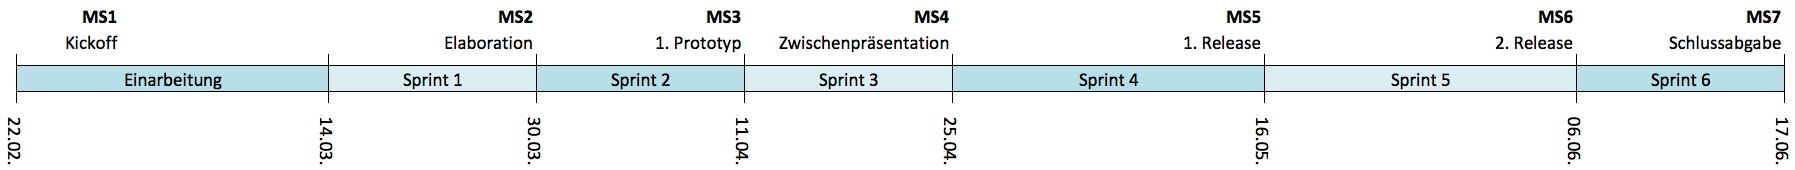
\includegraphics[width=\textwidth]{images/projektmanagement/zeitstrahl_v1.png}
	\caption{Erste Grobfassung des Projektplans als Zeitstrahl dargestellt}
	\label{image-project-plan-timeline1}
\end{figure}

Beim dritten Sprint wurde festgestellt, dass die Planung zu optimistisch und dass eine Veröffentlichung zum geplanten Zeitpunkt unrealistisch war. 
Die Planung wurde neu besprochen und in einem neuen \hyperref[image-project-plan-timeline2]{Zeitstrahl} festgehalten. 
Es gab Schwierigkeiten bei der Evaluation der Architektur und der Libraries. 
Die Libraries und Komponenten wurden in einzelnen Projekten getestet. 
Das hat uns zu einem besseren Verständnis für \brand{React Native} und damit zu neuen Erkenntnissen für die \hyperref[tb-evaluation-architektur]{Architekturentscheidung} verholfen. 

Erst beim \hyperref[pm-ms5]{Meilenstein 5} konnte eine Version mit den definitiv evaluierten Komponenten entstehen. 
Beim achten Meeting (29.04.2016) wurde mit unserem Betreuer, Herr Prof. Stefan Keller, besprochen, dass wir das Projekt nach der Abgabe gerne weiterführen würden.
Somit sollte es dann auch möglich sein, die App zu veröffentlichen.

Bis zum Ende vom \hyperref[pm-ms6]{Meilenstein 6} entstand ein erstes Release, eines Prototyps mit der geplanten Grundfunktionalität. 
Bei der Abgabe ist das Projekt in einem Zustand, bei dem sich neue Features zügig implementieren lassen.
Dieser aktuelle Stand zu Beginn des Projekts für den \hyperref[pm-ms5]{Meilenstein 5} geplant gewesen.

Somit ist dieser neue Projektplan entstanden.

\begin{figure}[H]
	\centering
	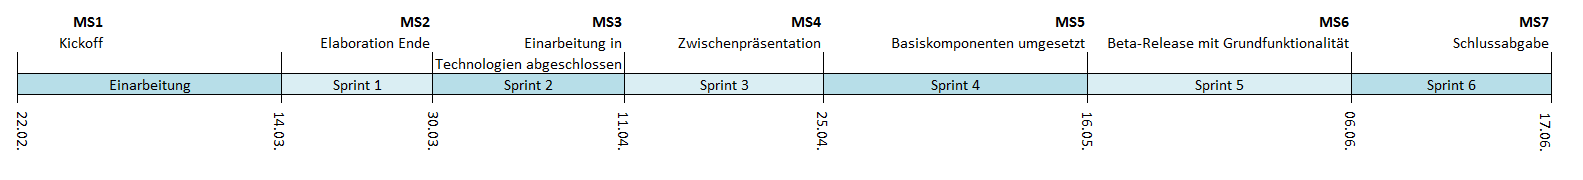
\includegraphics[width=\textwidth]{images/projektmanagement/zeitstrahl_v2.png}
	\caption{Überarbeiteter Projektplan als Zeitstrahl dargestellt}
	\label{image-project-plan-timeline2}
\end{figure}


\section{Sprints}
Durch die Anwendung von Scrum-Ansätzen wurden Sprints geplant. 
Eine Sprint-Periode dauerte immer bis zum Ende eines Meilensteins. 
Zu Beginn eines Sprints wurde das konkrete Vorgehen geplant und am jeweiligen Ende sind die Schwerpunkte dokumentiert worden.


\subsection{Sprint 1}
\textbf{14.03.2016 bis 30.03.2016}

Zum Schwerpunkt in diesem Sprint gehörte die Einarbeitung in die verwendeten Technologien und die Einarbeitung in das bestehende \kort{}-Projekt.

\subsection{Sprint 2}
\textbf{30.03.2016 bis 11.04.2016}

Im zweiten Sprint wurden die benötigten Libraries evaluiert und getestet.
Die Details und die Begründungen zu den Entscheidungen wurden im \hyperref[tb-evaluation]{Kapitel Evaluation} festgehalten.

\subsection{Sprint 3}
\textbf{11.04.2016 bis 25.04.2016}

Neben der Vorbereitung der Zwischenpräsentation wurden die Anforderungen aktualisiert. 
Das Ersetzen der Validierung im Frontend kam neu dazu. 
Zukünftige Arbeiten und Ideen wurden ebenfalls gesammelt und im \hyperref[pd-weiterentwicklung-realistisch]{Kapitel Realistische Arbeiten} dokumentiert.

\subsection{Sprint 4}
\textbf{25.04.2016 bis 16.05.2016}

Am Anfang des 4. Sprints wurde abgeklärt, ob ein Webprototyp mit \brand{React} umsetzbar ist. 
Dies stellte sich dann aber als zu aufwendig heraus. 
Die Idee (für eine folgende Studienarbeit) einer \brand{React}-\gls{WebApp} wurde abgewiesen.
Am Ende des Sprints wurde festgelegt, was getestet werden muss.

\subsection{Sprint 5}
\textbf{16.05.2016 bis 06.06.2016}

Während diesem Sprint fand das Meeting mit den Projektpartnern (Jürg Hunziker und Stefan Oderbolz) statt, um die Authentifizierung abzuklären. 
Es ging darum, neu zu evaluieren, wie das Login in der App umgesetzt wird und was dies für Änderungen am Backend mit sich bringen würde. 
Am Ende von Sprint 5 wurde ein Code Freeze bis zum Abgabetermin eingeleitet.

\subsection{Sprint 6}
\textbf{06.06.2016 bis 17.06.2016}

Die Validationen konnten im Frontend anhand von Anpassung der Businesslogik abgeschafft werden.
Ausserdem konnte die wichtige Internationalisierung für die Sprachen Englisch und Deutsch umgesetzt werden. 



\section{Meilensteine}
\label{pm-meilensteine}

In diesem Projekt wurde die Planung auf neun Meilensteine (MS) aufgeteilt. 
Die Meilensteine \hyperref[pm-ms8]{MS 8} und \hyperref[pm-ms9]{MS 9} finden nach der offiziellen Schlussabgabe statt und sind deswegen noch ohne Resultate dokumentiert.

\subsection{MS1: Kickoff}
\label{pm-ms1}
\textbf{Fällig am 25.02.2016}
\subsubsection{Resultate}
\begin{itemize}
	\item Kickoff Meeting bei Liip mit den Projektpartnern (Jürg Hunziker und Stefan Oderbolz) und dem Betreuer (Prof. Stefan Keller)
\end{itemize}

\subsection{MS2: Ende Elaboration}
\label{pm-ms2}
\textbf{Fällig am 29.03.2016}
\subsubsection{Resultate}
\begin{itemize}
	\item Infrastruktur aufgesetzt
	\begin{itemize}
		\item Datenbank
		\item \gls{CI}
		\item \brand{UserVoice}
		\item Redmine
		\item Installationsskripte
		\item Dokumentation aufgesetzt
	\end{itemize}
	\item Ausgangslage definiert und dokumentiert
	\item Anforderungsspezifikation erarbeitet
	\item Risikomanagement analysiert und dokumentiert
	\item Projektplan erarbeitet
	\item Map Komponente ausgewählt und eingesetzt
	\item Aufgabenstellung erarbeitet
	\item Testspezifikation erarbeitet
	\item Einarbeitung in die \kort{}-\gls{WebApp}
	\item \gls{GUI}-Mockups
\end{itemize}

\subsubsection{Erledigte Arbeiten}
Eine erste Version der Aufgabenstellung konnte erarbeitet werden. 
Die Dokumentation wurde eingeleitet.
Es gelang uns einen automatisierten Build der App aus dem \brand{GitHub}-Sourcecode mit \brand{Travis CI} aufzusetzen.
Für die Map-Komponente wurde die MapBox GL \gls{Library}\footnote{\url{https://libraries.io/npm/react-native-mapbox-gl}} mit den Vektor Daten von osm2vectortiles\footnote{\url{http://osm2vectortiles.org/}} evaluiert und getestet.
Nebenbei konnten wichtige Erfahrungen in den verwendeten Technologien (\brand{JavaScript}, \brand{React} und \brand{React Native}) gemacht werden.
Zusätzlich wurde ein für \brand{Android} angepasstes Design entworfen und Grundkonzepte der Architektur erarbeitet.
Die Architektur ist noch nicht final. 
Sie erleichtert uns aber den Einstieg beim Programmieren.
Die Infrastruktur ist soweit aufgesetzt.

\subsubsection{Probleme}
Für die detaillierte Erarbeitung der Testspezifikation fehlte noch die nötige Erfahrung in \brand{React Native}.


\subsection{MS3: Evaluation der Komponenten}
\label{pm-ms3}
\textbf{Fällig am 08.04.2016}
\subsubsection{Resultate}
\begin{itemize}
	\item Einarbeitung in \brand{JavaScript}, \brand{React} und \brand{React Native}
	\item \brand{Android} Prototyp
	\begin{itemize}
		\item Tab-Navigation
		\item Darstellung der Karte
		\item Evaluation der Architektur und Implementation des Grundgerüstes
		\item Missionen auf Map anzeigen
		\item Authentifizierung mit \gls{OAuth} evaluiert
	\end{itemize}
	\item \brand{Travis-CI} Konfiguration aktualisieren
\end{itemize}

\subsubsection{Erledigte Arbeiten}
Die Entwicklungsumgebung wurde optimiert. Das \brand{Travis}-Konfigurationsfile prüft den Code nun mit \brand{ESLint}\footnote{\url{http://eslint.org/}} (\brand{JavaScript} linter, prüft Styleguidelines) und \brand{flow}\footnote{\url{http://flowtype.org/}} (static type checker). 

Für die Tab-Navigation konnte eine Demo mit react-native-router-flux\footnote{\url{https://github.com/aksonov/react-native-router-flux}} umgesetzt werden. Diese muss noch in der \kort{} App implementiert werden. 

\gls{OAuth} (nur clientseitig, ohne Backend Kommunikation) wurde evaluiert und konnte dann anhand einer Demo getestet werden -- allerdings nur mit \brand{Facebook} und \brand{Google}.

Die Darstellung der Karte aus \nameref{pm-ms2} wurde leicht ausgebaut. Neu wird nun der Standort des Benutzers ermittelt.

Die Missionen konnten im Umkreis von fünf Kilometern geladen werden.

\subsubsection{Probleme}
Schwierigkeiten traten vor allem im Zusammenhang mit \brand{React Native} auf.
Oft gab es Build-Fehler bei gleicher Code-Basis.
Die Fehlerbehandlung hat uns enorm viel Zeit gekostet und es war schwer, im Internet Hilfestellungen zu erhalten.
Da \brand{React Native} alle zwei Wochen ein Update erhält, sind die Dokumentationen oder die Diskussionen im Internet teilweise schon wieder veraltet.\newline
Im Austausch mit anderen \brand{React Native} Entwicklern haben wir dasselbe Feedback erhalten.\newline
Der Prototyp konnte nicht wie geplant fertiggestellt werden und einige Arbeiten mussten auf den nächsten Meilenstein ausgelagert werden.

Die Authentifizierung mit dem Backend konnte noch nicht umgesetzt werden.

\subsection{MS4: Zwischenpräsentation}
\label{pm-ms4}
\textbf{Fällig am 22.04.2016}
\subsubsection{Resultate}
\begin{itemize}
	\item \brand{Mapbox} Prototyp fertig
	\begin{itemize}
		\item Missionen mit Marker auf Karte dargestellt
		\item Tab-Navigation implementiert
	\end{itemize}
	\item Zwischenpräsentation (Dauer ca. 30 Minuten)
	\begin{itemize}
		\item Aufgabenstellung, Problembesprechung
		\item IST-Situation
		\item geplantes Resultat
		\item Beschlussprotokoll für den \hyperref[pm-team]{Betreuer}
	\end{itemize}
\end{itemize}

\subsubsection{Erledigte Arbeiten}
Der Prototyp enthielt die Karte in einer Tab-Ansicht. 
An den jeweiligen Positionen der geladenen Missionen konnten Marker eingefügt werden.
Durch einen Klick auf einen Marker konnte der Titel der Mission erfolgreich in die Konsole geloggt werden.

Leider konnte noch immer keine Lösung für die Implementation eines Logins mit \gls{OAuth} 1.0a (\brand{OSM}) gefunden werden.
Dieses Feature noch zur Abgabe zu liefern wäre unrealistisch.
Deswegen wurde es auf den \hyperref[pm-ms9]{Meilenstein 9: Release für App Store} verschoben.

\subsubsection{Probleme}
Weiterhin traten Schwierigkeiten mit willkürlichen Fehlern der \brand{React Native} App auf. 
Aus diesen Gründen konnte die Navigation und die Struktur der App nicht abschliessend umgesetzt werden.
Dass der Benutzer nach dem Login automatisch zur Tab-Ansicht weitergeleitet wurde, hatte aufgrund eines Fehlers in der Navigations-\gls{Library} nicht geklappt.
Zwischenzeitlich wurde aus diesem Grund das Erhalten des Login-Tokens nach der Authentifizierung über \brand{Google} und \brand{Facebook} in einer separaten App getestet.


\subsection{MS5: Basis-Komponenten umgesetzt}
\label{pm-ms5}
\textbf{Fällig am 20.05.2016}
\subsubsection{Resultate}
\begin{itemize}
	\item Native Location Tracking implementiert
	\item \gls{GUI} fertig entworfen
	\item Testing-\gls{Framework} aufgesetzt
	\item Architektur-Entscheid und -Implementation
	\item Token basierte \brand{Google}-Authentifizierung im Frontend umgesetzt, nachdem das Backend vom Projektpartner, Stefan Oderbolz und Jürg Hunziker, dafür angepasst wurde
	\item \kort{}-Datenbank für Tests lokal aufgesetzt
	\item \kort{} ist \brand{iOS}-fähig
	\item \brand{React}-\gls{WebApp} evaluiert
	\item Validierungen vom Backend als Missionen laden
	\item Kurzvideo-Konzept besprochen
\end{itemize}

\subsubsection{Erledigte Arbeiten}

Wir haben die Architekturvarianten evaluiert und uns für die \brand{Flux}-Architektur entschieden.
Daraufhin wurde das bestehende -- noch sehr schlanke -- Grundgerüst, welches mit dem MVC-Pattern umgesetzt wurde, durch \brand{Flux} ersetzt.

Unterdessen konnte das Grundgerüst des \gls{GUI} grösstenteils fertiggestellt werden. 
Es fehlte noch die dynamische Behandlung von gewissen GUI-Komponenten.
Zum Beispiel die Unterscheidung, ob beim Lösen einer Mission ein Picker zum Auswählen der Antwort gerendert wird, oder ob ein Text-Input-Feld angeboten wird.

\kort{} konnte erfolgreich auf \brand{iOS} getestet werden. 

\subsubsection{Probleme}
Weiterhin war es nicht möglich mit der Router-Flux-Navigationskomponente eine Weiterleitung nach erfolgreichem Login zur Kartenansicht umzusetzen.
Hierbei handelte es sich um den bekannten Fehler dieser Komponente.
Das verzögerte leider das geplante Ziel: eine Mission zu lösen.

Die \kort{}-Datenbank konnte nur bei einem Entwickler richtig aufgesetzt werden. 
Es gab Probleme mit der Installation der Scripts auf \brand{OS X}.
Aus diesem Grund wurde für Tests nach Absprache mit dem Projektpartner (Jürg Hunziker), das Development-\kort{}-Backend genutzt.

\subsection{MS6: Beta-Release mit Grundfunktionalität}
\label{pm-ms6}
\textbf{Fällig am 06.06.2016}
\subsubsection{Resultate}
\begin{itemize}
	\item dynamische \gls{GUI} fertiggestellt
	\item Login Weiterleitung
	\item Login-Logik mit Local Storage
	\item Testing abgeschlossen
	\item Missionen und Validierungen sind lösbar
	\item Internationalisierung umgesetzt
\end{itemize}

\subsubsection{Erledigte Arbeiten}
Durch eine zusätzliche App-Loader-View konnte das Problem der Weiterleitung nach dem Login behoben werden.
Diese Komponente lädt nun alles im Voraus und erst danach wird je nach Zustand, ob der Benutzer eingeloggt ist oder nicht, die entsprechende Ansicht angezeigt.
Nach und nach wurden die Platzhalter der GUI mit dynamischen Daten der Businesslogik ersetzt. 
Die GUI ist nun dynamisch und zeigt je nach Zustand einer \inlinecode{Component} die entsprechende Oberfläche. 

Schlussendlich konnten wir erfolgreich Missionen und Validierungen lösen.


\subsubsection{Probleme}
Im \gls{Backend} sind Fehler aufgetreten wenn Validierungen negativ beantwortet wurden. 


\subsection{MS7: Schlussabgabe}
\label{pm-ms7}

\textbf{Fällig am 17.06.2016}

\subsubsection{Resultate}

\begin{itemize}
	\item Gebundene, vollständige Dokumentation eingereicht
	\item CD mit Abgabe eingereicht
	\item Abstract eingereicht
	\item Poster eingereicht
\end{itemize}


\subsection{MS8: Schlusspräsentation}
\label{pm-ms8}

\textbf{Fällig am 29.06.2016}

\subsubsection{Ziele}

\begin{itemize}
	\item Aktualisierte Dokumentation
	\item Design Verbesserungen
	\item Präsentation fertiggestellt
	\item Handouts ausgedruckt
\end{itemize}

\subsubsection{Resultate}

\begin{itemize}
	\item Dokumentation aktualisiert und neue CD gebrannt
	\item \brand{iOS} App getestet
\end{itemize}

\subsubsection{Probleme}
Bei der \brand{iOS} App funktioniert der Login mit \brand{Google} noch nicht. 
Es liegt ein Problem mit dem erhaltenen Token von \brand{Google} vor.

\subsection{MS9: Release für App Store}
\label{pm-ms9}

\textbf{Fällig am 05.07.2016}

\subsubsection{Ziele}

\begin{itemize}
	\item \brand{Android} App im \brand{Google Play} Store veröffentlicht
\end{itemize}


%Projektmonitoring
\chapter{Projektmonitoring}
\label{pm-projektmonitoring}

\section{Zeitanalyse}
\label{pm-zeitanalyse}
Für eine Bachelorarbeit werden 12 ECTS-Punkte vergeben, wobei ein Punkt einem Aufwand von 30 Stunden entspricht.
In einem Team von zwei Entwicklern, entspricht dies 360 Stunden Aufwand pro Person (siehe Tabelle \ref{pm-arbeitsaufwand}).

\begin{table}[H]
\centering
\label{pm-arbeitsaufwand}
\begin{tabular}{|l|r|}
\hline 
\multicolumn{1}{|c|}{\textbf{Person}} & \multicolumn{1}{|c|}{\textbf{Aufwand}} \\
\hline 
Marino Melchiori & 461.5 h \\
\hline 
Dominic Mülhaupt & 467 h \\  
\hline 
\end{tabular}
\caption{Arbeitsaufwand pro Person}
\end{table}

Wenn die gleich folgenden Tabellen \ref{pm-arbeitsaufwand-aktivität-mm} und \ref{pm-arbeitsaufwand-aktivität-dm} verglichen werden, ist die Arbeitsaufteilung sehr gut erkennbar. 
Dies ist in den Unterschieden des Aufwandes in den Aktivitäten Analyse, Implementation, Dokumentation und Testing erkennbar. 
Bei neuen Erfahrungen haben sich die Entwickler ausgetauscht und waren so immer auf dem aktuellen Stand. 

\begin{table}[H]
\centering
\begin{tabular}{|l|r|}
\hline
\multicolumn{2}{|l|}{\textbf{Marino Melchiori}} \\
\hline
\multicolumn{1}{|c|}{\textbf{Aktivität}} & \multicolumn{1}{|c|}{\textbf{Aufwand}} \\
\hline
Analyse \& Design & 106.00 h \\
\hline
Implementation & 125.00 h \\
\hline
Dokumentation & 141.00 h \\
\hline
Requirements & 30.75 h \\
\hline
Deployment & 16.25 h \\
\hline
Allgemein & 16.75 h \\
\hline
Projektmanagement & 25.75 h \\
\hline
\end{tabular}
\caption{Aufwand pro Aktivität (Marino Melchiori)}\label{pm-arbeitsaufwand-aktivität-mm}
\end{table}

\begin{table}[H]
\centering
\begin{tabular}{|l|r|}
\hline
\multicolumn{2}{|l|}{\textbf{Dominic Mülhaupt}} \\
\hline
\multicolumn{1}{|c|}{\textbf{Aktivität}} & \multicolumn{1}{|c|}{\textbf{Aufwand}} \\
\hline
Analyse \& Design & 49.50 h \\
\hline
Implementation & 191.75 h \\
\hline
Dokumentation & 66.25 h \\
\hline
Requirements & 26.00 h \\
\hline
Deployment & 7.00 h \\
\hline
Allgemein & 52.50 h \\
\hline
Projektmanagement & 52.00 h \\
\hline
Testing & 22.00 h \\
\hline
\end{tabular}
\caption{Aufwand pro Aktivität (Dominic Mülhaupt)}\label{pm-arbeitsaufwand-aktivität-dm}
\end{table}


\subsection{Soll-Ist-Zeitvergleich}
Die Tabelle \ref{pm-arbeitsaufwand-kategorie-ges} zeigt, wie das Projekt kategorisiert wurde. 
In der \kort{} \textit{Projekt}-Kategorie ging es vor allem um die Implementation der Architektur und die Verwendung und Einrichtung von \brand{React Native}. 
Die Kategorien \textit{Login}, \textit{Missionen}, \textit{Profil} und \textit{Highscore} enthalten die Implementation des \gls{GUI}. 
\textit{Map} und \textit{Internationalisierung} sind Kategorien, bei denen es um die Installation der entsprechend verwendeten \glslink{Library}{Libraries} ging. 
In der Kategorie \textit{Technologien} wurde die Einarbeitungszeit gebucht. 
Die \textit{Qualitätssicherung} beinhaltet das Testing und die Kategorie \textit{Allgemein} die Evaluation von verwendeten Konzepten und \glslink{Library}{Libraries}.

Die Schätzung fand jeweils bei der Erstellung eines Tickets in einer Kategorie statt. 

Die Differenz der \textit{Kort Projekt}-Kategorie lässt sich durch die häufigen Build-Fehler erklären. 
Das Suchen nach Lösungen im Internet war sehr zeitaufwendig. 

Bei der Kategorie \textit{Missionen} wurden 15 Stunden zu viel geschätzt. 
In diesem Fall setzten wir vermehrt auf \gls{Pair Programming}, da es sich dort um eine der ersten umgesetzten Funktionen handelte.
Somit konnte kostbare Zeit, die für das Refactoring geplant war, eingespart werden. 
Später folgende Features der Kategorien \textit{Login}, \textit{Profil} und \textit{Highscore} wurden viel besser geschätzt.

Schlussendlich wurden 21 Stunden zu viel geschätzt, was bei einem Arbeitstag von 8 Stunden etwa 2.5 Arbeitstagen entspricht. 


\begin{table}[H]
\centering
\begin{tabular}{|l|r|r|r|}
\hline
\multicolumn{4}{|l|}{\textbf{Soll-Ist-Vergleich vom Gesamtaufwand der Kategorien}} \\
\hline
\multicolumn{1}{|c|}{\textbf{Kategorie}} & \multicolumn{1}{|c|}{\textbf{Soll-Aufwand}} & \multicolumn{1}{|c|}{\textbf{Ist-Aufwand}} & \multicolumn{1}{|c|}{\textbf{Differenz}}\\
\hline
Kort Projekt & 71.75 h & 88.25 h & +16.50 h \\
\hline
Login & 91.50 h & 92.50 h & +1.00 h \\
\hline
Map & 47.75	h & 45.50 h & -2.25 h \\
\hline
Missionen & 59.75 h & 44.75 h & -15.00 h \\
\hline
Highscore & 11.50 h & 12.70 h & +1,20 h \\
\hline
Profil & 18.00 h & 16.25 h & -1.75 h \\
\hline
Technologien & 182.50 h & 187.55 h & +0.05 h \\
\hline
Gamification und Design & 7.25 h & 4.75 h & -2.50 h \\
\hline
Qualitätssicherung & 36.50 h & 30.00 h & -6.50 h \\
\hline
Internationalisierung & 4.50 h & 4.25 h & -0.25 h \\
\hline
Dokumentation & 204.00 h & 198.25 h & -5.75 h \\
\hline
Allgemein & 152.75 h & 144.50 h & -8.25 h \\
\hline
Meeting & 61.75 h & 59.25 h & -2.50 h \\
\hline
\textbf{Total} & \textbf{975.00 h} & \textbf{926.50 h} & \textbf{-21.00 h} \\
\hline
\end{tabular}
\caption{Soll-Ist-Vergleich: Gesamtaufwand pro Kategorie}\label{pm-arbeitsaufwand-kategorie-ges}
\end{table}

\section{Code-Statistik}
Zur groben Einschätzung der Grösse vom Projekt wurde in der Tabelle \ref{pm-cloc} die Gesamtanzahl der \brand{JavaScript} Codezeilen (ohne Code-Kommentare) gezählt. 
Beim Linken von \glslink{Library}{Libraries} gab es auch Anpassungen im \brand{Android}- und \brand{iOS}-Projekt. 
Der Umfang dieser Änderungen wurde nicht dokumentiert, da es sich vor allem um Anpassungen an vorhandenen Dateien handelte. 

\begin{table}[H]
\centering
\begin{tabular}{|l|r|}
\hline 
\textbf{Sprache} & \multicolumn{1}{|c|}{\textbf{Zeilen}} \\ 
\hline 
\brand{JavaScript} & 3913 \\
\hline 
\end{tabular}
\caption{Dateien und Codezeilen}\label{pm-cloc}
\end{table}

Die Tabelle \ref{pm-package-cloc} zeigt die Anzahl an Codezeilen in einem Package. 
Die Packages \inlinecode{Actions}, \inlinecode{Data}, \inlinecode{Dispatcher}, \inlinecode{DTO} und \inlinecode{Stores} sind von der verwendeten Architektur gegeben. 
\inlinecode{Constants} beinhaltet Konstanten, IDs und sonstige fixe Parameter. 
Im Package \inlinecode{Components} befinden sich die \gls{GUI}-Komponenten. 
Die \inlinecode{Shared Components} enthalten Buttons und weitere Komponenten, die oft wiederverwendet wurden. 

\begin{table}[H]
\centering
\begin{tabular}{|l|r|}
\hline 
\textbf{Package} & \multicolumn{1}{|c|}{\textbf{Zeilen}} \\ 
\hline 
\textit{Components} & 1042 \\
\hline 
\textit{Shared Components} & 463 \\
\hline 
\textbf{Total Components} & \textbf{1511} \\
\hline 
\textit{Actions} & 267 \\
\hline 
\textit{Data} & 513 \\
\hline 
\textit{Dispatcher ohne Tests} & 2 \\
\hline 
\textit{Dispatcher Tests} & 43 \\
\hline 
\textit{DTOs ohne Tests} & 199 \\
\hline 
\textit{DTO Tests} & 69 \\
\hline 
\textit{Stores ohne Tests} & 408 \\
\hline 
\textit{Store Tests} & 466 \\
\hline 
\textbf{Total Logik ohne Tests} & \textbf{1389} \\
\hline 
\textit{Constants} & 441 \\
\hline 
\end{tabular}
\caption{Codezeilen pro Package}\label{pm-package-cloc}
\end{table}


% -----------------------------------------
% FOOT
% -----------------------------------------
% Neue Seite beginnen
\cleardoublepage

% Anhänge
\part{Anhänge}

% Inhalt der CD
%\chapter*{Inhalt der CD}
% Titel auch in Kopfzeile anzeigen
\markboth{Inhalt der CD}{Inhalt der CD}
% Kapitel in Inhaltsverzeichnis einfügen
\addcontentsline{toc}{chapter}{Inhalt der CD}

\begin{forest}
  l sep+=1em,
  for tree={
    font=\sffamily,
    text=white,
    text width=15cm,
    minimum height=0.4cm,
    if level=0
      {fill=root}
      {fill=folder1},
    rounded corners=4pt,
    grow'=0,
    child anchor=west,
    parent anchor=south,
    anchor=west,
    calign=first,
    edge={root,rounded corners,line width=1pt},
    edge path={
      \noexpand\path [draw, \forestoption{edge}]
      (!u.south west) +(7.5pt,0) |- (.child anchor)\forestoption{edge label};
    },
    before typesetting nodes={
      if n=1
        {insert before={[,phantom]}}
        {}
    },
    fit=band,
    s sep=8pt,
    before computing xy={l=10pt},
  }
[/
  [Dokumentation/, for tree={fill=folder1}
    [Kort Reloaded - Marino Melchiori und Dominic Mülhaupt.pdf, for tree={fill=folder2}]
    [Anhänge/, for tree={fill=folder2,inner sep=3}
      [Abstract.pdf, for tree={fill=folder3}]
      [Aufgabenstellung.pdf , for tree={fill=folder3}]
      [Eigenständigkeitserklärung.pdf , for tree={fill=folder3}]
      [Einverständniserklärung Publikation auf eprints.pdf , for tree={fill=folder3}]
      [Gamified Mobile App für die Verbesserung von OpenStreetMap - Jürg Hunziker und Stefan Oderbolz.pdf , for tree={fill=folder3}]
      [Poster.pdf, for tree={fill=folder3}]
      [Schlusspräsentation.pdf, for tree={fill=folder3}]
      [Diagramme/, for tree={fill=folder3}]
      [Organisatorisches/, for tree={fill=folder3}]
      [Sitzungsprotokolle/, for tree={fill=folder3}]
    ]
  ]
  [Kort/, for tree={fill=folder1}
	[Sourcecode/, for tree={fill=folder2,inner sep=3}
	  [Kort\char`_0.1/, for tree={fill=folder3}]
	  [Kort\char`_0.2/, for tree={fill=folder3}]
	]
	[Kort\char`_0.2.apk, for tree={fill=folder2}]
  ]
  [Video/, for tree={fill=folder1}
	[Kort\char`_Movie.mp4, for tree={fill=folder2}]
  ]
]
\end{forest}

% Glossar
\printglossary[style=altlist,title=Glossar,toctitle=Glossar]
\label{glossar}

% Literaturverzeichnis
\bibliographystyle{plainurl}
%\bibliography{foot/literatur}

% Abbildungsverzeichnis
\listoffigures

% Tabellenverzeichnis
\listoftables

\end{document}